% Mestre em LaTeX - v0.5
% Copyleft 2008-2013 Bruno C. Vellutini - http://organelas.com/
%
% Ou seja, utilize e modifique os arquivos como desejar.
% 
% Para mais informações visite http://nelas.github.com/mestre-em-latex/

% Classe do documento
\documentclass[twoside,a4paper,11pt]{report}
\usepackage[english,brazil,brazilian]{babel}
\usepackage{caption}
\usepackage{cancel}
\usepackage{subfig}
\usepackage[section]{placeins}

%The placeins package gives the command \FloatBarrier, which will make sure any floats will be put in before this point.
\usepackage{placeins} % put this in your pre-amble

%The flafter package ensures that floats don't appear until after they appear in the code.
\usepackage{flafter}  % put this in your pre-amble


\usepackage{tikz,xcolor}
\usetikzlibrary{shapes,arrows}

\usepackage{circuitikz, ifthen}
\usepackage{amsmath}

% Pacotes e comandos customizados
\include{Config/meta}
%\usepackage[disable]{todonotes}

\usepackage{enumerate}
\usepackage{multirow}
%\usepackage{svg}

\usepackage{longtable}

\graphicspath{{./Figs/}}

\newcommand{\executeiffilenewer}[3]{%
	\ifnum\pdfstrcmp{\pdffilemoddate{#1}}%
	{\pdffilemoddate{#2}}>0%
	{\immediate\write18{#3}}\fi%
}

\newcommand{\includesvg}[1]{%
\executeiffilenewer{#1.svg}{#1.pdf}%
{inkscape -z -D --file=./Figs/#1.svg %
--export-pdf=./Figs/#1.pdf --export-latex}%
\input{./Figs/#1.pdf_tex}%
}

% Início do texto
\begin{document}



%\tableofcontents
% Desenvolvimento de mancal magnético para rodas de reação

% Limpa cabeçalhos.
% (solução para lidar com a númeração das páginas pré-textuais).
\pagestyle{empty}

%% Capa
%\begin{titlepage}
%
%% Se quiser uma figura de fundo na capa ative o pacote wallpaper
%% e descomente a linha abaixo.
%% \ThisCenterWallPaper{0.8}{nomedafigura}
%
%\begin{center}
%{\LARGE \nomedoaluno}
%\par
%\vspace{200pt}
%{\Huge \titulo}
%\par
%\vfill
%\textbf{{\large São Paulo}\\
%{\large \the\year}}
%\end{center}
%\end{titlepage}

% Faz com que a página seguinte sempre seja ímpar (insere pg em branco)
\cleardoublepage

% Numeração em elementos pré-textuais é opcional (ativada por padrão).
% Para desativá-la comente a linha abaixo.
\pagestyle{fancy}

% Números das páginas em algarismos romanos
\pagenumbering{roman}

%% Página de Rosto

% Numeração não deve aparecer na página de rosto.
\thispagestyle{empty}

\begin{center}
{\LARGE \nomedoaluno}
\par
\vspace{200pt}
{\Huge \titulo}
\end{center}
\par
\vspace{90pt}
\hspace*{175pt}\parbox{7.6cm}{{\large  \textbf{Texto apresentado a Escola Politécnica da Universidade de São Paulo para o Exame de Qualificação de Mestrado em Engenharia de Sistemas}}}%Documento de Qualificação apresentado ao Instituto de Biociências da Universidade de São Paulo, para a obtenção de Título de Mestre em Ciências, na Área de XXXXXXXX.}}

\par
\vspace{1em}
\hspace*{175pt}\parbox{7.6cm}{{\large Orientador: Prof. Dr. José Jaime da Cruz}}

\par
\vfill
\begin{center}
\textbf{{\large São Paulo}\\
{\large \the\year}}
\end{center}

\newpage

%% Ficha Catalográfica
%\hspace{8em}\fbox{\begin{minipage}{10cm}
%Aluno, Nome C.
%
%\hspace{2em}\titulo
%
%\hspace{2em}\pageref{LastPage} páginas
%
%\hspace{2em}Dissertação (Mestrado) - Escola Politécnica da Universidade de São Paulo. Departamento de Controle e Automação.
%
%\begin{enumerate}
%\item Mancal Magnético
%\item Roda de Reação
%\item Controle Multivariável
%\end{enumerate}
%I. Universidade de São Paulo. Escola Politécnica. Departamento de Eletrônica.
%
%\end{minipage}}
%\par
%\vspace{2em}
%\begin{center}
%{\LARGE\textbf{Comissão Julgadora:}}
%
%\par
%\vspace{5em}
%\begin{tabular*}{\textwidth}{@{\extracolsep{\fill}}l l}
%\rule{16em}{1px} 	& \rule{16em}{1px} \\
%Prof. Dr. 		& Prof. Dr. \\
%Nome			& Nome
%\end{tabular*}
%
%\par
%\vspace{10em}
%
%\parbox{16em}{\rule{16em}{1px} \\
%Prof. Dr. \\
%José Jaime da Cruz
%}
%\end{center}
%
%%\newpage
%
%%% Dedicatória
%%% Posição do texto na página
%%\vspace*{0.75\textheight}
%%\begin{flushright}
%%  \emph{Dedicatória...}
%%\end{flushright}
%
%\newpage
%
%%% Epígrafe
%%\vspace*{0.4\textheight}
%%\noindent{\LARGE\textbf{Exemplo de epígrafe}}
%%% Tudo que você escreve no verbatim é renderizado literalmente (comandos não são interpretados e os espaços são respeitados)
%%\begin{verbatim}
%%
%%
%%\end{verbatim}
%%\begin{flushright}
%%Lenine e Bráulio Tavares
%%\end{flushright}
%
%\newpage
%
%% Agradecimentos
%
%% Espaçamento duplo
%\doublespacing
%
%\noindent{\LARGE\textbf{Agradecimentos}}
%
%Agradeço ao meu orientador, ao meu co-orientador, aos meus colaboradores, aos técnicos, à seção administrativa, à fundação que liberou verba para minhas pesquisas, aos meus amigos, à minha família....

\newpage

\vspace*{10pt}
% Abstract
\begin{center}
  \emph{\begin{large}Resumo\end{large}}\label{resumo}
\vspace{2pt}
\end{center}
% Pode parecer estranho, mas colocar uma frase por linha ajuda a organizar e reescrever o texto quando necessário.
% Além disso, ajuda se você estiver comparando versões diferentes do mesmo texto.
% Para separar parágrafos utilize uma linha em branco.
\noindent

	Roda de reação é um sistema excecional para o controle de atitude de satélites, \todo{continuar}
	
	Devido as consequências de qualquer fricção no movimento relativo entre a inércia (parte rotativa) e o satélite (estator) o mancal torna-se um componente crítico da roda de reação. A fricção se traduz não apenas num maior consumo de potência elétrica, como também na introdução de uma zona morta de atuação em torque, bem como na limitação da vida útil da roda de reação devido ao gradual desgaste do mancal. 
	
	Mancais magnéticos são alternativas aos mancais tradicionais (esferas, lubrificação seco) pois trabalham sem contato mecânico entre o rotor e o estator minimizando assim a fricção entre ambas as partes. Além da minimização do atrito, o ganho em confiabilidade e vida útil da roda de reação é considerável por não apresentar desgastes mecânicos.
	 
	Esta dissertação a vem ao encontro de projetar um mancal magnético para rodas de reação com aplicação na malha de controle de atitude de satélites. Propomos uma topologia diferente da encontrada na literatura, com um oito polos e dois graus de liberdade ativo.
	 
	 
\par
\vspace{1em}
\noindent\textbf{Palavras-chave:} Mancal Magnético, Rodas de Reação, Modelagem Eletromagnética
\newpage
%
%% Criei a página do abstract na mão, por isso tem bem mais comandos do que o resumo acima, apesar de serem idênticas.
%\vspace*{10pt}
%% Abstract
%\begin{center}
%  \emph{\begin{large}Abstract\end{large}}\label{abstract}
%\vspace{2pt}
%\end{center}
%
%% Selecionar a linguagem acerta os padrões de hifenação diferentes entre inglês e português.
%\selectlanguage{english}
%\noindent
%		Este trabalho vem ao encontro de projetar um mancal magnético para rodas de reação que tem utilização na malha de controle de atitude de satélites. \ldots
%\par
%\vspace{1em}
%\noindent\textbf{Keywords:} Magnetic Bearing, Reaction Wheel, Multivariable Control

% Voltando ao português...
\selectlanguage{brazilian}

\newpage

% Desabilitar protrusão para listas e índice
\microtypesetup{protrusion=false}

% Lista de figuras
\listoffigures

% Lista de tabelas
\listoftables

% Abreviações
% Para imprimir as abreviações siga as instruções em 
% http://code.google.com/p/mestre-em-latex/wiki/ListaDeAbreviaturas
\printnomenclature

% Índice
\tableofcontents

% Re-habilita protrusão novamente
\microtypesetup{protrusion=true}
   			    	
\begin{tabular}{|c|c|}
Símbolo &  Significado \\ 
\hline \hline

	$g_{ne}$	& Entreferro nominal externo \\
	$g_{ni}$	& Entreferro nominal interno \\

	$h_{fee}$	& Altura do ferro estator externo \\
	$h_{fei}$	& Altura do ferro estator interno \\
	$h_m$		& Altura do ímã \\
	$h_n$		& Altura do polo da bobina \\
	
	$r_{eei}$	& Raio do polo estator externo \\				
	$r_{re}$	& Raio do polo do ferro rotor \\		
	$r_{n}$		& Raio do polo da bobina \\		
	$r_{ei}$	& Raio do ferro estator interno \\	

	$w_{fee}$	& Largura do ferro estator externo\\
	$w_{fei}$	& Largura do ferro estator interno \\
	$w_{rf}$	& Largura do ferro rotor \\
	$w_{rr}$	& Largura do anel retorno rotor \\
	$w_m$		& Largura do ímã \\
	$w_n$		& Largura do polo da bobina \\

	$S_m$		& Área do ímã\\	
	$S_{ef}$	& Área do ferro estator externo \\
	$S_{rf}$	& Área do ferro rotor\\
	$S_{rr}$	& Área do anel retorno rotor\\
	$S_{ge}$	& Área do entreferro externo\\

	$\mathcal{F}_c$ & Fluxo magnético ímã 				\\
	$R_{p}$			& Relutância no íma 				\\
	$R_{ge}$		& Relutância entreferro externo 	\\
	$R_{ef}$		& Relutância ferro estator externo 	\\
	$R_{rf}$		& Relutância ferro rotor 			\\
	$R_{rr}$		& Relutância anel retorno rotor 	\\
	$R_{lm}$		& Relutância vazamento ímã 			\\
	$R_{lg}$		& Relutância vazamento entreferro externo \\

	$P_{lm}$		& Permeância do vazamento do ímã	\\

	$H_c$			& Coecirvidade do íma \\
	$H_m$			& Campo magnético efetivo ímã \\

	$B_r$ 			& Fluxo máximo fornecido pelo ímã \\
	$B_m$			& Vetor campo magnético efetivo ímã \\
	$B_{gx}$		& Vetor Campo magnético estator externo, componente x \\
	$B_{gz}$		& Vetor Campo magnético estator externo, componente z \\

	$\mu_0$			& Permeabilidade do vácuo \\
	$\mu_m$			& Permeabilidade do ímã \\
	$\mu_{ef}$		& Permeabilidade do ferro estator externo \\
	$\mu_{rf}$		& Permeabilidade do ferro rotor \\
	$\mu_{rr}$		& Permeabilidade do anel retorno rotor\\

	$F_{ex}$		& Força de atração em x devido o estator externo \\
	$F_{ez}$		& Força de atração em y devido o estator externo \\
\end{tabular} 
	

\fancyhead{}
% Número da página do lado esquerdo [L] nas páginas ímpares [O] e do lado direito [R] nas páginas pares [E]
\fancyhead[LO,RE]{\thepage}
% Nome da seção do lado direito em páginas ímpares
\fancyhead[RO]{\nouppercase{\rightmark}}
% Nome do capítulo do lado esquerdo em páginas pares
\fancyhead[LE]{\nouppercase{\leftmark}}
% Limpar os campos do rodapé
\fancyfoot{}
% Omitir linha de separação entre cabeçalho e conteúdo
\renewcommand{\headrulewidth}{0pt}
% Omitir linha de separação entre rodapé e conteúdo
\renewcommand{\footrulewidth}{0pt}
% Altura do cabeçalho
\headheight 13.6pt

		
% Faz com que o ínicio do capítulo sempre seja uma página ímpar
\cleardoublepage

% Inclui o cabeçalho definido no meta.tex
\pagestyle{fancy}

% Números das páginas em arábicos
\pagenumbering{arabic}

\chapter{Introdução}\label{intro}

Os sistemas de controle de atitude e órbita são uma das tecnologias mais críticas de qualquer sistema espacial. O desenvolvimento de um sistema de controle de atitude em território nacional permanece incompleto \citep{Veloso2009} e a venda de seus componentes ao nosso país é, frequentemente, recusada por países detentores dessa tecnologia.

Basicamente, um sistema de controle de atitude é formado por sensores, atuadores e uma central responsável pelo processamento dos sinais dos sensores e comando dos atuadores, segundo uma lei de controle. Os sensores mais comuns são detectores de horizonte, sensores magnéticos, sensores solares, giroscópios e rastreadores estelares. 

Os principais atuadores incluem: propulsores, torques magnéticos e rodas de reação. A quase totalidade destes componentes de controle possui atualmente alguma iniciativa de desenvolvimento no país, seja por instituições governamentais ou por grupos de pesquisa independentes \citep{PresidenciaRepublica}. A principal exceção são as rodas de reação que praticamente não tem projetos de desenvolvimento em andamento e, no entanto, representam um componente indispensável na realização de manobras, na estabilização e no controle de atitude em três eixos. 

Rodas de reação são dificilmente substituíveis pois apresentam larga faixa de operação em torque (ao contrário de atuadores magnéticos) e são alimentadas pela energia renovável fornecida por painéis solares (ao contrário de propulsores baseados em um estoque finito de combustível). Por estes motivos, rodas de reação estão presentes em praticamente qualquer satélite que apresente requerimentos mínimos de desempenho em atitude.

Uma roda de reação pode ser descrita como um atuador inercial com funcionamento baseado no princípio de conservação do momento angular. A atuação da roda de reação sobre o satélite se realiza por intercâmbio do momento angular, limitado ao eixo de rotação da roda. Devido a grande diferença entre a inercia do satélite e o da roda de reação, um controle de atitude com muita precisão é possível com esse sistema.

Rodas de reação são tipicamente constituídas de um motor elétrico, geralmente um motor sem escovas, um mancal e um elemento de inércia.  O elemento de inércia e o motor são montados sobre o mancal que deve garantir a  precisa rotação em torno de um eixo. A velocidade de rotação do sistema é controlada por uma eletrônica de acionamento do motor. Rodas de reação podem ser comandadas de duas maneiras distintas: por rotação ou por torque. Quando comandada por torque, a roda de reação deve ser capaz de estimar o torque útil gerado por ela (o torque efetivo menos as perdas). 

Fig. \ref{fig:EsquemaRoda} ilustra um esquema genérico de uma roda de reação. No caso, quatro são os subsistemas: eletrônica de acionamento, motor, mancal e inércia. A eletrônica é responsável pelo controle e pelo acionamento do motor que, por sua vez, possui um sensor de velocidade e um de corrente. 


\begin{figure}[ht!]
\centering
\includegraphics[width=1\linewidth]{./Figs/EsquemaRoda}
\caption{Esquema geral de uma roda de reação}
\label{fig:EsquemaRoda}
\end{figure}


O controle de atitude  com rodas de reação demanda que esse tipo de  atuador opere em toda sua escala de velocidade, inclusive na inversão de seu sentido de rotação (passagem pelo zero), de uma forma estável e controlada. Essa zona morta é efeito do atrito estático do mancal, minimizar esse efeito é essencial para o bom funcionamento da roda de reação. A zona morta pode ser compensada (no caso do mancal por rolamento) pela implementação de leis de controle com malhas de velocidade e corrente, além de um estimador de atrito.

O projeto de uma roda de reação começa pelo estudo do momento angular necessário para movimentar o satélite. Com o momento angular definido, especifica-se a inércia e então o mancal, por último projeta-se um motor capaz de rotacionar o conjunto mancal mais inércia.


\section{Objetivo}

Essa dissertação acompanha o esforço de projetar um mancal magnético para uma roda de reação que está sendo desenvolvida no Núcleo de Sistemas Eletrônicos Embarcados (NSEE) do Instituto Mauá De Tecnologia (IMT) com apoio do Instituto Nacional De Pesquisas Espaciais (INPE).

O projeto, envolve o desenvolvimento de uma topologia capaz de ser utilizada numa roda de reação para satélites de médio porte, mais especificamente, para a plataforma multi missão.


\section{Justificativa}

A suspensão do rotor com relação ao estator representa uma parte crítica em rodas de reação \citep{taniwaki2003experimental} devido as consequências de qualquer fricção no movimento relativo entre estes dois componentes. Com efeito, a fricção se traduz não apenas em um maior consumo de potência elétrica como também na introdução de uma zona morta de atuação em torque, bem como na limitação da vida útil da roda de reação devido ao gradual desgaste do mancal.

Uma solução mecânica para a interface entre o rotor e o estator é o mancal por rolamento. Apesar de sua aparente simplicidade, apresenta desafios para a obtenção dos valores mínimos de fricção necessários, em vista das exigências de consumo, controlabilidade e vida útil da roda de reação \citep{Krishnan2010}. No caso de aplicações aerospaciais, a lubrificação do rolamento representa também, considerável dificuldade devido à impossibilidade de utilização de lubrificantes tradicionais em condições de baixa ou nenhuma pressão atmosférica, que leva à perda dos componentes voláteis destes lubrificantes e sua consequente degradação. Outra dificuldade se deve à tendência de migração dos lubrificantes na ausência de gravidade, o que costuma ser abordado com estratégias de recaptura ou relubrificação. Sistemas de relubrificação, em particular, apresentam grande complexidade e seu comportamento orbital é de difícil validação em laboratório.

As dificuldades associadas ao uso de mancal de rolamento residem também em sua modelagem, consequência da variação de viscosidade do lubrificante em função da temperatura do mancal, o que torna o coeficiente de fricção dependente da velocidade de rotação e das condições térmicas em geral. O mancal por rolamento apresenta, por outro lado, grande vantagem construtiva devido à compactação do sistema e a não necessidade de eletrônica extra para o seu controle. 

Para contornar os problemas de lubrificação em baixa pressão, algumas rodas de reação  utilizam um sistema hermeticamente selado pressurizado com um gás inerte \citep{Krishnan2010}. Esta solução relaxa os requisitos de lubrificação, porém impõe uma força de arrasto extra na roda e não resolve o problema da migração dos lubrificantes na ausência de gravidade. Uma pesquisa detalhada dos lubrificantes de classe espacial e estratégias de selamento e relubrificação deve ser realizada.

Outra solução é a utilização de um mancal magnético \citep{Bangcheng2012}, que é uma alternativa sem contato mecânico entre o rotor e o estator, pela qual o rotor é mantido suspenso magneticamente. O ganho em confiabilidade e vida útil da roda de reação é considerável \citep{Marble2006}, sendo a vida útil basicamente limitada  pela durabilidade da eletrônica. A operação sem contato elimina a necessidade de lubrificante e possibilita consequentemente a operação em vácuo, o que se traduz em simplificação nos requisitos da concepção mecânica. 

A ausência de fricção elimina a zona morta de aplicação de torque em baixas velocidades, eliminando não-linearidades da lei de controle, além de possibilitar a eliminação de defeitos de balanceamento e vibrações mecânicas. Consequentemente, gera um ganho em simplicidade dos algoritmos e em desempenho do controle de atitude. A contrapartida é a adição de uma malha de controle para a suspensão eletromagnética. O ganho de eficiência trazido pela ausência de fricção também é contrabalanceado, ao menos parcialmente, pelo consumo de potência dos atuadores deste tipo de mancal.


\section{Revisão bibliográfica}


Estudo iniciais sobre mancais magnéticos são datados do século XIX \citep{Weise1989}, porém só recentemente começaram a ter grandes aplicações na sociedade. Essas aplicações vão desde motores de alta eficiência até equipamentos médicos. Mancais magnéticos fazem uso extensivo de campos magnéticos e tiveram uma grande evolução quando os ímãs de terras raras tornaram-se acessíveis, possibilitando o aumento da geração de campos magnéticos permanentes \cite{Furlani2001}.

Mancais magnéticos podem ser classificados em dois grandes grupos: os que utilizam da \textit{força de relutância} e os que utilizam da \textit{força de Loretz}. O primeiro grupo é chamado de mancais magnéticos ativos (na literatura AMBs) e o segundo são os mancais magnéticos passivos (PMBs) \cite{Schweitzer2009}.

Os AMBs funcionam com um controle ativo de algumas das forças atuantes no mancal a fim de estabilizar o sistema (controle em malha fechada). Já os mancais puramente passivos geram as forças necessárias para estabilizar o rotor apenas via ímãs.
Mancais magnéticos puramente passivos (seis graus de liberdade) que utilizam somente ímãs são impossíveis, dado que sempre um dos graus de liberdade torna-se instável (Teorema de Earnshaw's). \todo{corrigir: JU}

%Mancais híbridos, que operam com parte de seus graus de liberdade passivamente estáveis e parte de seus graus de liberdade ativamente estáveis possuem  



\subsection{Graus de liberdade}

Os mancais magnéticos podem ser classificados pelo número de graus de liberdade controlados ativamente \citep{Schweitzer2009}:

\begin{enumerate}[a)]
	\item  Mancal puramente passivo
	
	Este mancal totalmente passivo é formado por um rotor contendo um conjunto de imãs permanentes em disposição de Halbach \citep{Detoni2012}, o que gera potencialização do campo magnético adjacente ao rotor. Um conjunto de enrolamentos passivos no estator é excitado por esse campo magnético girante. Na eventualidade de qualquer deslocamento do rotor, o enrolamento reage com o campo magnético, gerado pela atração/repulsão do rotor, ocasionando a volta à posição de equilíbrio. O sistema é estável a partir de uma velocidade de rotação mínima do rotor (velocidade crítica). O fato desta topologia não funcionar em baixas velocidades angulares a torna pouco adaptada para aplicação em rodas de reação.
	
	\item  Mancal ativo num grau de liberdade
	
	Neste caso, o rotor e o estator são formados por ímãs permanentes em configuração repulsiva, tornando o sistema estável axialmente. O eixo radial é instável e necessita controle ativo, normalmente realizado por meio de eletro-ímãs. Trata-se de uma configuração que necessita de uma eletrônica de controle relativamente simples e de baixo consumo de potência. No entanto, a ausência de controle ativo radial tende a gerar oscilações mecânicas de difícil amortecimento.
	
	\item Mancal ativo em dois graus de liberdade
	
	Aqui, o rotor e o estator compõem um circuito magnético em configuração atrativa, em geral com ímãs permanentes no rotor acoplados a um circuito magnético de baixa relutância no estator. O sistema é estável axialmente mas necessita controle ativo nos dois eixos radiais. Essa configuração resulta num mancal de boa rigidez radial, com arquitetura simplificada e pequenas dimensões, principalmente na direção axial.
	
	\item Mancal ativo em cinco graus de liberdade
	
	Este mancal totalmente ativo é formado por atuadores eletromagnéticos nas duas direções radiais, na direção axial e nos dois modos de rotação radiais. A principal vantagem de sua aplicação em rodas de reação é a possibilidade de atuação em mais de um eixo de rotação, devido à capacidade de manobra do componente de inércia. Trata-se no entanto de um sistema de controle de grande complexidade, com consequente redução de confiabilidade. 
\end{enumerate}

\subsection{Topologias com Aplicação em Rodas de Reação}

Encontramos na literatura três topologias distintas para utilização de mancais magnéticos em rodas de reação. Os mancais propostos para esse tipo de aplicação possuem, em sua maioria, dois graus de liberdade ativos e fazem uso de ímãs permanentes para a geração de campos magnéticos para minimizar o consumo elétrico ativo do sistema. Em seguida, analisamos os principais pontos desses mancais.

A topologia proposta por \citet{Bernus1998} trabalha com dois graus de liberdades ativos, com ímãs permanentes no rotor e dois estatores: um interno com bobinas para o controlo do fluxo magnético no rotor (por consequência na direção radial) e outro externo para estabilização axial que também contribui com a rigidez axial. 

Nessa topologia (Fig. \ref{Fig:modelo:frances}), um fluxo magnético contínuo é gerado no rotor por ímãs permanentes ali instalados, as bobinas instaladas no estator interno conseguem gerar campos aditivos e subtrativos no rotor (dependente do sentido da corrente). Se o campo for aditivo, pode-se aumentar a rigidez do eixo axial, caso o campo for subtrativo, consegue-se diminuir sua rigidez, tornando assim mais fácil o deslocamento radial do rotor.

\begin{figure}[!ht]
	\centering
	\includegraphics[width=1\linewidth]{./Figs/mancais/frances}
	\caption{Corte da topologia proposta por \cite{Bernus1998} \\
	a: estator externo; b: rotor; c: estator interno; d: ímãs permanentes}
	\label{Fig:modelo:frances}
\end{figure}

A topologia proposta por \citet{Scharfe2001} difere por ter somente um estator e pelos ímãs permanentes estarem localizados no estator e não no rotor. Como ilustrado na Fig. \ref{Fig:modelo:alemao}. 

%\todo[inline]{falar mais ...}

\begin{figure}[!ht]
	\centering
	\includegraphics[width=0.8\linewidth]{./Figs/mancais/alemao.pdf}
	\caption{Corte da topologia proposta por \cite{Scharfe2001} \\
	a: estator externo; b: rotor; c: estator interno; d: ímãs permanentes}
	\label{Fig:modelo:alemao}
\end{figure} 

Com essa arquitetura é possível utilizar as bobinas tanto para exercer uma força atrativa no rotor quanto para tornar a sua rigidez mas branda, facilitando a atração do rotor. É possível também aumentar a rigidez axial por permitir a inserção um fluxo positivo em ambas as bobinas, esse fluxo soma-se com o fluxo gerado pelos ímãs permanentes.

Mais recentemente, uma nova arquitetura foi proposta por \citet{Bangcheng2012} para ser utilizado em uma roda de reação de um satélite ágil.  O rotor é composto de duas partes, uma externa utilizada para estabilizar o mancal na direção axial e outra interna para controle de posição na direção radial. Diferente das outras propostas, essa não utiliza um perfil em "C" para estabilização dos graus de liberdade passivos, mas sim, faz uso de um perfil plano com ímãs permanentes tanto no rotor quanto no estator.  Ímãs permanentes também são usados nos polos do mancal, esses criam um fluxo (\textit{bias}) constante diminuindo a corrente necessária para controlar o rotor.
 
%\begin{figure}[!ht]
%	\centering
%	\includegraphics[width=1\linewidth]{./Figs/mancais/chines}
%	\caption{Corte da topologia proposta por \cite{Bangcheng2012}}
%	\label{Fig:modelo:chines}
%\end{figure}

\subsection{Modelagem Eletromagnética}

Devido as não linearidades do mancal magnético (por exemplo a sua rigidez em função do deslocamento), a modelagem analítica é de difícil obtenção e uma análise por elementos finitos é recomendada \citep{pilat2007automatic}. Com esse tipo de análise é possível verificar o acoplamento das forças e momentos envolvidos além das características térmicas do sistema.

Modelos analíticos \cite{Tezuka2013, Chiba} auxiliam no entendimento e na escolha dos parâmetros construtivos e magnéticos do mancal. A solução de um modelo analítico quando comparada a de um modelo com elementos finitos é computacionalmente mais rápida.

Com o modelo analítico é possível a utilização de métodos de otimização \citep{Wu2009, Fang2014} para a obtenção de um mancal com melhores propriedades, dentre elas, menor potência, maior rigidez e dimensões dentro das especificações. 

\subsection{Sensoriamento}

Devido ao controle da posição do rotor em mancais magnéticos, o sensoriamento de sua posição é essencial para o funcionamento do sistema. Duas linhas de sensoriamento são encontradas na literatura: Mancais auto sensoreados \citep{Vischer1993} e os que utilizam sensores de posição dedicados para esse fim.

Os mancais magnéticos sem sensores (\textit{sensorless}) utilizam geralmente as bobinas de seus polos para sensorear a posição do rotor. Diversas técnicas podem ser empregadas \citep{Hofer2009a, Mukhopadhyay2005} entre elas: medição da indutância dos polos pela injeção de um sinal com uma portadora de frequência mais elevada ou a medição da força contra-eletromotriz induzida nas bobinas.
 
Já os mancais sensoreados utilizam sensores de deslocamentos exclusivos para a medição da posição do rotor e, por consequência, do tamanho do entreferro \cite{boehm1993sensors}. Os sensores podem ser de dois tipos, capacitivos ou indutivos, dependendo do material construtivo do sistema. Opera-se geralmente com sensores na distribuição diferencial, visando minimizar os efeitos de suas não linearidades.
 
\subsection{Mancais auxiliares}

 Mancais auxiliares são importantes em mancais magnéticos, pois são eles que evitam colisões entre as partes fixas e as rotativas em caso de algum tipo de falha. Mancais magnéticos projetados para operar em altas rotações não possuem bom rendimento na inicialização  (baixa rotação) e se utilizam dos mancais auxiliares nessa zona até atingirem a sua velocidade de operação. Os mancais auxiliares podem ser compostos por rolamentos esféricos \citep{Sun2004a} ou por elementos sólidos auto lubrificante como Teflon.
 
\subsection{Técnicas de controle}

O controle de mancais magnéticos é uma área fértil da engenharia de controle, as não linearidades do sistema tornam os projetos nada triviais.  

Técnicas de controle clássicas são utilizadas com bastante frequência em mancais magnéticos. Controle do tipo PID  \citep{Tezuka2013} possue boa robustez. O controle  do tipo \textit{feedforward} é utilizado em casos onde há o acoplamento entre os graus de liberdade, podendo ser utilizado para o desacoplamento dos graus de liberdade. Outras técnicas propostas na literatura vão de encontro ao controle multivariável como controle robusto \citep{Jimenez-Lizafrraga2007}, controle ótimo \citep{Schuhmann2012} e controle não linear \citep{Rundell1996}.


\section{Metodologia}

A metodologia adotada neste trabalho envolve a utilização de simulações em elementos finitos para o desenvolvimento das partes magnéticas do mancal, uma modelagem fenomenológica foi feita para a realização da otimização dos parâmetros físicos do sistema. 

O desenvolvimento do projeto foi executado como ilustrado na Fig. \ref{fig:metodologia:fluxo:dev}, onde primeiramente as especificações de projeto foram levantadas e uma topologia de mancal proposta com base no levantamento bibliográfico. 

Um protótipo foi construído a fim de avaliar a topologia proposta, verificou-se com ele que as premissas de estabilidade e força foram alcançadas. A construção desse protótipo foi realizada na oficina mecânica da Escola de Engenharia Mauá (EEM), devido a ausência de fomento, a prototipagem não pode ser efetuada seguindo todas as especificações de rigor mecânico, o que gerou falhas na montagem.

O material utilizado também foi influenciado por esse fator, utilizou-se no caso o aço 1020 para as partes magnéticas (de amplo uso comercial) e alumínio para as partes não magnéticas. 

Na etapa de otimização, dividiu-se o projeto em duas partes: na primeira considerou-se somente a parte passiva (estator externo e rotor) até que um conjunto com rigidez suficiente na direção axial e com menor força de atração na direção radial fosse atingido. Com esses valores buscou-se um estator interno capaz de exercer força de atração suficiente no rotor para estabilizá-lo em seu ponto de operação.

Com um modelo em elementos finitos (FEM) calculou-se com exatidão os parâmetros magnéticos do mancal proposto a serem utilizados na modelagem dinâmica do rotor.

Com o modelo dinâmico, um controlador capaz de estabilizar o rotor em seu ponto de operação foi proposto, com ele, provou-se a controlabilidade do mancal nas restrições de potência propostas. 


 
\begin{figure}[th!]
	\centering
	\includegraphics[width=1\linewidth]{Figs/metodologia_fluxo_dev}
	\caption{Fluxo de desenvolvimento}
	\label{fig:metodologia:fluxo:dev}
\end{figure} 
 
\section{Sumário Estruturado}
 
No segundo capítulo, o mancal magnético proposto foi descrito e suas propriedades construtivas apresentadas. Nele podemos verificar conceitualmente todos os componentes que constituem o sistema proposto.

O capítulo três apresenta um modelo não linear para representar a interação entre o estator externo e o rotor. Esse conjunto é responsável pela estabilização do rotor nos graus de liberdades passivamente estáveis. No modelo analítico foi aplicada uma otimização nos parâmetros construtivos do mancal visando encontrar um mancal compacto e com boa rigidez passiva. A partir de um modelo em elementos finitos obteve-se as relações de força por deslocamento.

Na quarta parte desta dissertação, um modelo fenomenológico que modela a interação entre o estator interno e o rotor está apresentado. Similarmente ao capítulo anterior, foi aplicada uma otimização visando a obtenção dos parâmetros construtivos do estator interno. Com o modelo em elementos finitos, chega-se às equações de força resultante dessa otimização do mancal.  

No quinta capítulo, a partir das dimensões e das equações de forças definidas anteriormente, um modelo dinâmico para o rotor está apresentado. Esse modelo foi utilizado para o projeto de uma malha de controle capaz de estabilizar o rotor em seu ponto de operação.

O último capítulo constituí-se por uma revisão do desenvolvimento da dissertação e pela apresentação de considerações finais sobre o projeto.


				
\pagestyle{empty}
\cleardoublepage
\pagestyle{fancy}

\chapter{Mancal magnético}

%\begin{small}
%\begin{itemize}
%	\item especificações
%		\begin{itemize}
%			\item massa 
%			\item dimensões
%			\item consumo 
%			\item potência máxima
%		\end{itemize}
%	\item restrições
%	\item introdução da topologia do mancal
%	\item estator externo
%		\begin{itemize}
%			\item ímãs 
%			\item perfil em C
%			\item ferro
%			\item 
%		\end{itemize}
%	\item estator interno
%		\begin{itemize}
%			\item bobinas
%		\end{itemize}
%	\item batente
%	\item base
%	\item fixação ?
%	\item modelo em elementos finitos
%\end{itemize}
%\end{small}


Rodas de reação são constituídas basicamente de um motor, mancal, elemento de inércia e eletrônica de controle. O motor e o mancal são considerados os sistemas mais críticos, influenciando diretamente a qualidade da roda de reação e o cumprimento dos requisitos. Nesse projeto de pesquisa, buscou projetar um mancal magnético que possa fazer parte de uma roda de reação para satélites de médio porte. Para tanto é necessário que o mancal satisfaça os requisitos impostos para uma roda de reação, tais como: desbalanceamento, consumo, velocidade e atrito.

O mancal magnético proposto deve satisfazer as especificações da Tabela \ref{tab:PMM:especificações}, onde deseja-se atingir os requisitos de uma roda de reação para um satélite de classe II, baseado nos dados da plataforma multimissão (PMM) do INPE \citep{Veloso2009}, possibilitando que o mesmo possa rejeitar pertubações orbitais e executar manobras de posicionamento. 
%\cite{junior2005estudo}\todo{cite}. 

\begin{table}[!ht]
    \centering
    \begin{tabular}{l c l }
		Parâmetro & Valor &   \\
       	\hline \\
 		Torque   						  & 0,1 & [Nm]  \\
 		Momento angular  				  & 10 &      [Nms] \\
 		Rotação 							  & $\pm4000$ & [rpm] \\
 		Oscilação do torque 				  & 10  & [\%] \\
 		Torque de fricção do mancal 		  & 0,01 & [Nm] \\
 		\multirow{2}{*}{Desbalanceamento residual} & 0,2 & [g.cm]\\
 		 & 20  & [g.cm$^{2}$]  \\
 		\multirow{3}{*}{Consumo de potência} 
 		& 3 & [W] 	 \\
 		& 30 & [W] \\
 		& 100 & [W] 	\\	
 		Tensão de alimentação  & 20 à 40 & [V]  \\
    \end{tabular}
    \caption{Especificações de requisito da roda de reação}
    \label{tab:PMM:especificações}
\end{table}

O acionamento da roda de reação deve ser possível em ambos os sentidos de rotação e com a mesma eficiência. Requer também que o eixo de rotação tenha inclinação menor do que 0,1 grau com relação a superfície de fixação da roda. A precisão de alinhamento é necessária para a adequada atuação da roda de reação no eixo sob controle.

A roda de reação deve ter dimensões limitadas em 250mm de diâmetro por 100mm de altura com massa total que não deve exceder 4kg. Na concepção das partes construtivas da roda de reação será considerada a necessidade de operação contínua por longos períodos de tempo (em torno de quatro anos).

\section{Visão Geral}

% [Scharfe2001]
% Magnetic bearings can be realised by using attractive or repulsive forces. A better mass vs. stiffness ratio can be achieved by using the attractive force mode. Preference was given to the 2 DOF option where the wheel is actively controlled along two orthogonal radial directions where axial movements and all other degrees of rotor freedom are passively controlled by means of permanent magnets, except for the rotor spin. The two radial axes are independently controlled by their control loops. This design principle generally results in a flatter geometry, using less volume and being suitable for panel mounting. Moreover, the two DOF actively controlled bearing allows a high momentum-to-mass ratio of the wheel as parts of the bearing contribute to the momentum storage capacity. For position detection, magnetic field displacement type inductive sensors are mounted with 90 degrees angular spacing around the flywheel, facing the rim surface.

O mancal magnético proposto nesse trabalho é em partes uma junção das topologias propostas por \citet{Bernus1998} e \citet{Scharfe2001}. O mancal possui quatro graus de liberdade passivamente estáveis: \textit{tilt, row, pitch} e sua direção axial, os outros dois graus de liberdade (as translações radias) são estabilizados ativamente. O torque imposto para a rotação do rotor não é abordado nesse trabalho mas será desenvolvido por um motor elétrico de corrente contínua sem escovas (BLDC), instalado no interior do mancal.

O circuito magnético do mancal é composto por dois estatores: um interno ao rotor, outro externo e um rotor. O estator externo é responsável pela estabilização dos graus de liberdade passivos já o interno por possibilitar o controle das posições radiais. Optou-se por instalar os ímãs no estator externo visando um maior fluxo magnético nos modos passivamente estáveis do mancal, além de visar o melhor balanceamento do rotor (se compararmos com a instalação do ímãs no rotor. A Fig. \ref{fig:mancal:topo} ilustra o mancal proposto. O rotor é a parte móvel do mancal e onde é fixado a parte móvel do motor. Adotou-se uma geometria plana visando uma melhor rigidez nos modos instáveis do mancal, possibilitando também a montagem em modo painel. Optou-se por um mancal externo ao motor  para conseguir uma rigidez dentro dos limites de massa e dimensões e que atingisse as especificações  da roda de reação. 

\begin{figure}[ht!]
\centering
%\includegraphics[width=0.6\linewidth]{./Figs/mancais/mancal:topo}
\includegraphics[width=0.6\linewidth]{./mancais/modelo-elementos-finitos}
\caption[Corte ilustrativo do mancal magnético]{Perspectiva das partes magnéticas do mancal}
\label{fig:mancal:topo}
\end{figure}

A Fig. \ref{fig:mancal:corte} ilustra um corte radial no mancal proposto, verificamos que os ímãs permanentes estão localizados no estator externo, criando um fluxo magnético que circula pelo rotor e estabiliza o eixo axial.

Mancais magnéticos podem ser projetados para usar forças magnéticas atrativas ou repulsivas. Uma melhor relação massa/ rigidez pode ser alcançada pela utilização de forças magnéticas atrativas, e esse é o papel das bobinas localizadas no estator interno. Oito núcleos são utilizados para exercer força de atração suficiente no rotor para mover da posição de equilíbrio (rotor batido) e estabilizar no ponto de operação. 

\begin{figure}[ht!]
	\centering
	\includegraphics[width=1\linewidth]{./Figs/mancais/mancal_corte}
	\caption[Corte ilustrativo do mancal magnético]{Corte ilustrativo do mancal magnético. Onde: a) estator externo, b) rotor, c) estator interno, d) ímã permanente, e) bobinas}
	\label{fig:mancal:corte}
\end{figure}

Um batente foi projetado para evitar que as partes magnéticas (metálicas) se choquem em caso de falha na malha de controle ou em situações em que o sistema encontra-se desligado. O batente limita a excursão máxima do rotor em seus graus de liberdade: axial, radial e \textit{tilt}. O Batente não interfere no circuito magnético do sistema e é localizado no estator externo. Toda parte fixa do sistema é fixa em uma base também não magnética.

Uma eletrônica de acionamento, sensoriamento e processamento é alocada na parte inferior da base, tornando o sistema compacto. A eletrônica possui \textit{drivers} para controle das correntes nas bobinas e também um sistema de sensoriamento para medir a posição do rotor. Um sistema microprocessado é proposto para realizar o controle e gestão do sistema.

% O mancal é composto dos seguintes subsistemas:
%
%\begin{itemize}
%	\item estator Interno
%	\item estator Externo
%	\item rotor
%	\item batente
%	\item base
%	\item eletrônica
%\end{itemize}

\section{Estator externo}\label{cap:mancal:estator:externo}

O estator externo, responsável pela estabilização dos graus de liberdade passivamente estáveis e é formado de três partes : ferro topo, ímãs, ferro base. A combinação dessas partes faz com que o estator tenha uma secção em formato de C. Os ferros (topo e base) servem para guiar o campo magnético através do gap e pelo rotor. 

O circuíto magnético de uma secção do estator externo é ilustrado na Fig. \ref{Fig:mancal:circuito:passivo}. Verificamos que o fluxo magnético gerado pelo ímã permanente busca o caminho com menor relutância para fechar o circuito magnético. Esse caminho ocorre pelos ferros do estator externo, passando então pelo entreferro e  pelo rotor.

\begin{figure}[!ht]
	\centering
	\def\svgwidth{1\columnwidth}
	\includesvg{mancal_passivo_circuito}
	\caption{Circuíto magnético do estator externo}
	\label{Fig:mancal:circuito:passivo}
\end{figure}

Podemos identificar nesse circuito, seis principais relutâncias, sendo elas :

\begin{itemize}
	\item $R_{ímã}$ : Relutância do ímã permanente
	\item $R_{ft}$ : Relutância devido ao ferro topo
	\item $R_{gt}$ : Relutância do entreferro superior
	\item $R_{fb}$ : Relutância devido ao ferro base
	\item $R_{gb}$ : Relutância do entreferro inferior	
\end{itemize}

Além das relutâncias, temos como fonte geradora de campo magnético o ímã localizado entre os ferros : $F_{ima}$. Devido ao fluxo magnético permanente o rotor sofre atração em ambos os lados, se no ponto de equilíbrio, ou seja, com um entreferro simétrico em ambos os lados, a força resultante tenderia ser nula e o rotor permaneceria em equilíbrio no ponto de operação (criticamente estável). 

Esse modo de operação é chamado diferencial e possibilita que a força resultante no rotor devido aos ímãs permanentes torne-se linear. Para tanto projetamos o estator externo do mancal para trabalhar em sempre com o ferro saturado, na saturação a relação densidade fluxo magnético e campo magnético torna-se praticamente constante para pequenas variações de campo magnético. Com isso a componente da força que é proporcional ao quadrado do campo magnético torna-se praticamente constante. Além da linearização obtêm-se um aumento na rigidez axial sem um grande aumento na rigidez radial, o que exigiria uma maior energia da parte ativa para a estabilização.

No caso de um deslocamento axial ocorre um aumento no comprimento do entreferro e por consequência em sua relutância ($R_{g}$), essa condição foge da zona de menor energia gerando uma força restaurativa no rotor para restabelecer um circuito com menor relutância magnética.

A Fig. \ref{fig:modelo:circuito:passivo:forcas} demonstra as forças atuantes no rotor em dois cenários diferentes, na primeira (a) com o rotor no ponto de equilíbrio (com o mesmo entreferro ao longo de toda circunferência) e em (b) com o rotor deslocado axialmente, verificamos nesse caso que a resultante da força não é nula mas sim possui uma componente em y. Essa componente é a responsável pela estabilização dos graus de liberdade passivos.

\begin{figure}[th!]
\centering
\subfloat[rotor no ponto de equílibro]{
	\includegraphics[width=0.8\linewidth]{./Figs/modelo_circuito_passivo_forcas_a}
	} \\
\subfloat[rotor transladado axialmente]{
	\includegraphics[width=0.8\linewidth]{./Figs/modelo_circuito_passivo_forcas_b}
	}
\caption{Fluxo magnético no estator externo e rotor}
\label{fig:modelo:circuito:passivo:forcas}
\end{figure}

O circuito passivo deve possuir rigidez axial suficiente para manter o rotor alinhado em ambientes com gravidade (para validação na terra) e rigidez radial menor para um baixo gasto energético do circuito ativo na estabilização do rotor.

%\todo[inline]{o campo no ferro do estator externo e’ saturado mesmo, estava confundindo com o campo no estrator interno.
%no estator externo a saturação é necessária, pois maximiza o B absoluto e minimiza o efeito diferencial, o que aumenta a rigidez axial (passiva) sem aumentar muito a rigidez radial.}

%\todo[inline]{falar do tilt}

\section{Rotor}

O Rotor foi projetado com perfil em C e sofre tanto força de atração do estator externo quanto do estator interno, porém com campos em diferentes orientações. O rotor é projetado para que seu ferro trabalhe na zona de não saturação, a saturação nesse caso é indesejada pois limitaria o fluxo total que flui através dos circuitos magnéticos e também resultaria quando em rotação em uma região de possível aquecimento.

\section{Estator interno}

O estator interno é formado de oito polos distribuídos homogeneamente a cada 45 graus e interligados por um anel de circulação interno. Os polos funcionam como atuadores (eletroímãs) para a estabilização do roto no eixo radial (x, z),  cada polo é formado por um núcleo. Uma revolução de meio mancal é ilustrado na Fig. \ref{fig:modelo:mancal:estator:interno}. 

\begin{figure}[ht!]
	\centering
	\includegraphics[width=1\linewidth]{./Figs/modelo_mancal_estator_interno}
	\caption{Corte em perspectiva do estator interno}
	\label{fig:modelo:mancal:estator:interno}
\end{figure}

O estator interno foi concebido para atuar sempre com três polos ativos, essa abordagem faz com que o fluxo do campo magnético que percorre o rotor seja maximizado no eixo onde deseja-se realizar a atração. A Fig. \ref{fig:modelo:mancal:estator:interno:fluxo} mostra o estator interno com três de seus polos ativos: (A),(B),(C) e o fluxo que flui pelo rotor. Os polos (A) e (C) nesse exemplo trabalham com polaridade inversa ao (B) para forçar que o fluxo feche por B e não por nenhum outro polo, maximizando assim a força de atração $F_B$. Uma parte do fluxo do campo magnético não atravessa por (B) e fecha por outros polos. A corrente induzida em (A) e (C) é a metade da corrente no polo principal (B) isso é feito para evitar que o polo B atinja a saturação, já que o campo que o atravessa é composto pela totalidade do induzido em sua bobina mais a parte dos campos de (A) e (C).

\begin{figure}[ht!]
	\centering
	\includegraphics[width=0.7\linewidth]{./Figs/modelo_mancal_estator_interno_fluxo}
	\caption{Fluxo magnético}
	\label{fig:modelo:mancal:estator:interno:fluxo}
\end{figure}

As forças geradas $F_A$ e $F_C$ possuem componentes em x e y, as componentes y são de mesma intensidade e se cancelam, restando uma componente aditiva em x. A força resultantes são portanto:

\begin{align}
 	F_x &= F_B + F_{Ax} + F_{Cx} \\
 	F_y &= 0 = F_{Cy} - F_{Ay} 
\end{align}


Nesse modo de operação pode-se gerar uma força y e x, para isso pasta induzir da mesma maneira um novo campo em (H) e (G). 

O circuito magnético entre o estator interno e o rotor pode ser visto na Fig. \ref{fig:modelo:circuito:ativo:explicativo}, verificamos que o circuito é formado de quatro principais elementos : A bobina, fonte geradora de campo magnético (c), a relutância do entreferro que depende da distância entre os polos e o rotor (b), as relutâncias do ferro do rotor (a) e do ferro do anel de retorno (d).

\begin{figure}[ht!]
\centering
\includegraphics[width=0.7\linewidth]{./Figs/modelo_circuito_ativo_explicativo}
\caption[Circuito eletromagnético estator interno e rotor]{Circuito eletromagnético estator interno e rotor: (a) relutâncias do rotor, (b) relutâncias do entreferro, (c) }
\label{fig:modelo:circuito:ativo:explicativo}
\end{figure}

\section{Batente}

 O batente é necessário por duas razões principais: Evitar que partes metálicas colidam dado uma falha na estabilização do rotor; saturar  o tamanho do entreferro, limitando por consequência a força de atração máxima que é exercida sobre o rotor.  Essa limitação é necessária para a situação em que o rotor encontra-se mais afastado do ponto de operação, sem o limite do batente o entreferro se tornaria grande o que necessitaria de uma potência maior por partes das bobinas para estabilizar-lo no ponto de operação.  Além de limitar a máxima translação radial, o batente é responsável por limitar também a translação axial e sua inclinação (\textit{tilt}).
 
 A Fig. \ref{fig:mancal:batente:corte} é uma ilustração do batente proposto para o mancal magnético, é composto de duas partes: (a) responsável por limitar o entreferro máximo entre o rotor e o estator externo; (b) frange para limitar a inclinação do rotor. Encontra-se na literatura projetos de macais magnéticos com rolamentos. Essa escolha seria inadequada para o projeto já que a proposta é a aproximação de um projeto espacializável, a incorporação do rolamento demandaria um projeto específico.
 
Optou-se por instalar o batente no estator externo por duas razões distintas: facilidade na montagem pois  é o local onde possui maior entreferro (portanto espaço) e também para servir de fixação para unir os ímãs e os ferros do estator externo. 

\begin{figure}[th!]
\centering
\includegraphics[width=0.4\linewidth]{./Figs/mancais/mancal_batente_corte}
\caption{Ilustração do batente proposto}
\label{fig:mancal:batente:corte}
\end{figure}


%\begin{figure}[th!]
%\centering
%\includegraphics[width=0.5\linewidth]{./Figs/mancais/mancal:batente:3d}
%\caption{Perspectiva do batente proposto}
%\label{fig:mancal:batente:3d}
%\end{figure}

O batente deve ser rígido suficiente para aguentar possíveis impactos do rotor, veremos no Cap. \ref{Cap:Modelagem:Dinamica} que os essas forças são da ordem de centenas de Newtons. Propõem a utilização de Nylon ou Teflon na construção do batente devido a suas propriedades de lubrificação a seco. 

\section{Base}

As partes não móveis do mancal são fixas em uma base de propriedade não magnéticas (alumínio), a base serve para alinhar as partes do mancal e ao mesmo tempo possibilita a movimentação do rotor na direção axial e radial (dentro das especificações de oscilação). 

%\section{Eletrônica}
%
%A eletrônica proposta é composta de sistemas de potência para o acionamento das bobinas (polos), eletrônica de sensoriamento para medição das posições do rotor e uma eletrônica de controle (digital) onde é implementando o controle do sistema. 

%Um sistema microconrolado (ou FPGA) é proposto para implementação das leis de controle, o acionamento das bobinas será realizado através da modulação da largura de pulso (PWM).

\section{Dimensões}

Ao longo do desenvolvimento da dissertação, utilizou-se as nomenclaturas a seguir para descrever as dimensões que geram o mancal proposto. As nomenclaturas são esclarecidas na Fig. \ref{fig:modelo_dimensoes} e na Tabela \ref{tab:modelo:dimensoes:nomenclatura}.

\begin{table}[ht!]
	\centering
	\begin{tabular}{c l}
		Nomenclatura & Descritivo \\
		$h_{fee}$	& Altura do ferro estator externo \\
		$w_{fee}$	& Largura do ferro estator externo\\
		
		$h_m$		& Altura do ímã \\
		$w_m$		& Largura do ímã \\

		$g_{ne}$	& Entreferro nominal externo \\
		
		$w_{fr}$	& Largura do ferro rotor \\
		
		$g_{ni}$	& Entreferro nominal interno \\
		
		$h_n$		& Altura do polo da bobina \\
		$w_n$		& Largura do polo da bobina \\
		
		$w_{fei}$	& Largura do ferro estator interno \\
		$h_{fei}$	& Altura do ferro estator interno \\

		$r_{eei}$	& Raio do polo estator externo \\				
		$r_{re}$	& Raio do polo do ferro rotor \\		
		$r_{n}$		& Raio do polo da bobina \\		
		$r_{ei}$	& Raio do ferro estator interno \\		
		
	\end{tabular} 
	\caption{Valores iniciais, máximos e mínimos utilizado na otimização, valores em milímetros.}
	\label{tab:modelo:dimensoes:nomenclatura}
\end{table}


\begin{figure}[th!]
	\centering
	\includegraphics[width=0.8\linewidth]{Figs/modelo_dimensoes}
	\caption{}
	\label{fig:modelo_dimensoes}
\end{figure}

 \subsection{Modelo em Elementos Finitos}
 
 Foi utilizado como ferramenta de modelagem o Software de elementos finitos e multi física \textit{Comsol}. Nas simulações foram utilizados a curva de histerese do Aço 1020 , as simulações foram realizadas com uma solido tridimensional e a análise realizada foi a estacionária.  A Fig. \ref{Fig:Simulacao:Passivo:Mesh} ilustra a malha utilizada na execução das simulações com um número aproximado de 19000 elementos.
 
 \begin{figure}[!ht]
 	\centering
 	\includegraphics[width=0.5 \columnwidth,angle=0]{Figs/Simulacoes/Passivo/3D_Mesh=1,2.png}
 	\caption{Modelo Comsol do circuito passivo Malha utilizada nos cálculos}
 	\label{Fig:Simulacao:Passivo:Mesh}
 \end{figure}
 
Nas simulações em elementos finitos, o modelo criado possui físicas distintas para os diversos elementos do mancal. No caso dos ferros, aplicou-se a lei de Ampère com a relação construtiva \textbf{BH} interpolada de uma tabela. Nos componentes compostos por ar, a relação utilizada foi a linear $B=\mu_0 H$. 

Na simulação do ímã, utilizou-se a relação de magnetização : $B = \mu_0 (H + M)$ onde M é a magnetização do meio em A/m. Para as bobinas, o material utilizado foi o cobre e a equação para a densidade de corrente (J) aplicada foi: $ J = \frac{N I}{A}$, onde: $N$ é o número de espiras; $I$ a corrente total aplicada na bobina e $A$ a área da secção da bobina.



\section{Prototipagem}

Para prototipagem do mancal foi necessário a criação de nove diferentes peças para possibilitar a montagem do sistema. A proposta de montagem visa minimizar a influência no circuito magnético que alteraria o comportamento das forças no rotor mas ao mesmo tempo buscou-se um sistema simétrico e robusto.  A Fig. \ref{fig:montgem:corte} é um corte da estrutura proposta, verificamos que o estator interno (RW-M-EI) é formado por uma única peça, enquanto o rotor e o estator externo são fragmentados em mais de uma parte.

A localização e os tipos de parafuso (magnético, não magnético) foi uma decisão de projeto, optou-se por uma localização que minimiza-se a influência no circuito magnético. A Tab. \ref{Tab:nomenclatura:mancal} possui a descrição e nomenclatura das partes propostas para a prototipagem do mancal magnético.

 \begin{table}[ht!]
 	\centering
 	\begin{tabular}{l l}
 		Nomenclatura & Descrição  \\ \hline
 		RW-M-BA 		&	Base do mancal \\
 		RW-M-C   		 &	Casca externa\\
 		RW-M-EEB	  & Estator externo base\\
 		RW-M-EET & 	Estator externo topo\\
 		RW-M-BT & 	Batente\\
 		RW-M-RFB & 	Rotor ferro base\\
 		RW-M-RFT	&  Rotor ferro topo\\
 		RW-M-RN & 	Rotor núcleo\\
 		RW-M-EI	&  Estator interno\\
 	\end{tabular} 
 	\caption{Nomenclatura partes mancal}
 	\label{Tab:nomenclatura:mancal} 
 \end{table} 

 
A não utilização de materiais laminados propicia  a aparição de correntes induzidas  no circuito magnético quando exposto a correntes variantes no tempo. Essas correntes induzidas (Eddy) causam uma redução na força eletromagnética e aquecem o material, alterando a relação corrente/força utilizada como parâmetro para o projeto da lei de controle. Minimizar as correntes induzidas tornam o sistema mais eficiente porém a construção de um protótipo laminado é mecanicamente difícil. Outra solução é a utilização de "ferro leve" (\textit{soft iron}), que possui propriedades que limitam a criação de corrente induzida, em contrapartida esses materiais normalmente apresentam menor permeabilidade magnética e menor valor do campo magnético para atingir a saturação \citep{Han2013a}. O material escolhido para os circuitos magnéticos foi o Aço 1020 e para as partes não magnéticos utilizou-se alumínio.
  
\begin{figure}[th!]
\centering
\includegraphics[width=1\linewidth]{./mancais/montgem_corte}
\caption{Partes do mancal}
\label{fig:montgem:corte}
\end{figure}


	
\pagestyle{empty}
	\cleardoublepage
\pagestyle{fancy}


\chapter{Estator Externo e Rotor}

A parte passiva do mancal magnético, composta pelo estator externo e pelo rotor,  pode ser descrita como o circuito da Fig. \ref{Fig:Modelagem:circuito:passivo:umlado}, onde um ímã permanente gera um fluxo magnético ($\mathcal{F}_c$) que estabiliza o eixo axial (passivo). O caminho principal desse fluxo é através do entreferro ($R_{ge}$) tanto pelos ferros do estator ($R_{ef}$) quanto pelos ferros do rotor ($R_{rf}$ e $R_{rr}$). Dois caminhos extras são considerados, um de vazamento de fluxo magnético no ímã ($R_{lm}$) e outro em cada entreferro ($R_{lg}$). 

\begin{figure}[!ht]
	\centering
	\def\svgwidth{1\columnwidth}
	\includesvg{modelo_circuito_passivo_umlado}
	\caption{Circuito magnético passivo suposto}
	\label{Fig:Modelagem:circuito:passivo:umlado}
\end{figure}

Um modelo fenomenológico foi inicialmente criado e nele aplicado um algorítimo de otimização a fim de encontrar um mancal ótimo para um certo funcional que valoriza as especificações anteriores. Com as dimensões encontradas, um modelo em elementos finitos foi gerado e as constantes de força calculadas de maneira mais precisa.

\section{Modelagem Magnética}

Nesse modelo, o ímã é considerado como uma fonte de fluxo magnético na forma equivalente a um circuito Thevenin. A força magnética coerciva ($\mathcal{F}_c$) representa a força magnética necessária para levar o ímã permanente a produzir um fluxo magnético nulo. Ímãs de terra rara (Samário Cobalto - Neodímio), possuem tipicamente uma curva linear de magnetização no segundo quadrante, essa curva depende de duas constantes físicas que variam com o material usado: $H_c$ constante que associa o comprimento do ímã com a força coerciva ($ F_c = H_c \, l_m$) e $B_r$ que descreve o fluxo máximo do ímã num cenário de curto circuíto ($\phi_r = B_r \, A_m$), ilustrada na Fig. \ref{Fig:Modelagem:circuito:passivo:ima}.

\begin{figure}[!ht]
	\centering
	\def\svgwidth{0.7\columnwidth}
	\includesvg{modelo_circuito_passivo_ima}
	\caption{Curva de desmagnetização típica de ímãs de terra rara}
	\label{Fig:Modelagem:circuito:passivo:ima}
\end{figure}

A curva de magnetização é descrita como :

\begin{align}
B_m = B_r + \frac{B_r}{H_c} H_m
\label{eq:p:ima}
\end{align}

A relação $\frac{B_r}{H_c}$ pode ser interpretada como a permeabilidade do meio (ímã) e possui tipicamente um valor próximo da permeabilidade do vácuo, $\mu_0$. O ponto de operação do ímã depende da curva de carga do circuíto magnético em que ele está inserido, para isso é necessário primeiramente calcular o valor da permeabilidade total e então identificar o ponto de operação do ímã e o seu fluxo produzido.

Considera-se nesse modelo para os materiais ferros magnéticos a curva de magnetização do ferro 1020, a curva não linear é apresentada na Fig. \ref{Fig:Modelagem:BH}, nota-se que a saturação ocorre por volta de 1.3T. Essa relação pode ser descrita como:

\begin{align}
B(H) = \mu(H) \, H
\label{eq:p:BH:ferro}
\end{align}

\begin{figure}[!ht]
	\centering
	\caption*{ Vetor campo magnético (T) x Campo Magnético (A/m)}
	\includegraphics[width=0.6\linewidth]{modelo_curva_bh}
	\caption{Curva de magnetização para o ferro 1020}
	\label{Fig:Modelagem:BH}
\end{figure}


\subsection{Campo Magnético no Entreferro}

A relutância magnética é proporcional ao comprimento da linha de campo no meio e inversamente proporcional a permeabilidade do meio e a área em que o campo está disperso. Com isso, calcula-se as relutância principais do circuíto :

\begin{align}
R_{p}  &= \frac{h_m}{\mu_m \, S_m}			\\
R_{ef} &= \frac{w_{ef}}{\mu_{ef}\, S_{ef}}  \\     
R_{rf} &= \frac{w_{rf}}{\mu_{rf}\, S_{rf}}   \\    
R_{rr} &= \frac{h_m}{\mu_{rr} \, S_{rr}}     \\      
R_{ge} &= \frac{g_{ne}}{\mu_0  \, S_{ge}}        
\end{align}


A permeância gerada pelo vazamento pode ser calculada por \citep{Leupold1996a}: 

\begin{align}
P_{lm} &= \frac{0.64 \,  \mu_0 \,r_{ee}}{h_m/(h_m+2h_{ef})+1} \\
R_{lg} &= P_1 + P_2 + P_3 + P_4	
\end{align} 

Sendo $R_{g//}$ a associação paralela entre a relutância do entreferro e o vazamento associado, $R_1$ a soma das relutâncias do circuíto principal e $R_T$ a associação entre todas as relutâncias do circuíto. $\phi_1$ é o fluxo magnético na primeira malha e $\phi_2$ o fluxo magnético na malha principal. Obtém-se as seguintes equações:

\begin{align}
\phi_m &= \phi_1 + \phi_2 \\
&= \frac{F_c}{R_p + R_T} \\
\mathcal{F}_c	 &= \phi_1 \, (R_p + R_1) \\
\mathcal{F}_c    &= \phi_2 \, (R_p + R_{lm})
\end{align}

Encontra-se o campo magnético efetivo no entreferro:

\begin{align}
\phi_{ge} &= \frac{\phi_1 \, R_{lg}}{R_{ge}+R_{lg}} \\
B_{ge} &= \frac{\phi_g}{S_{ge}}
\end{align}


\subsection{Decomposição do Vetor Campo Magnético B em X e Z} \label{SubSec:CampoX/Y}

O campo magnético acumulado no entreferro pode ser decomposto em componentes $B_x$ e $B_z$ que dependem do deslocamento do rotor em $\Delta_x$ e $\Delta_z$. Esse deslocamento implica também em um aumento no comprimento do entreferro: $l_g$. A Fig. \ref{Fig:modelo:passivo:DxDz} ilustra o deslocamento. Tal modelo não leva en consideração o \textit{tilt} do rotor, o que implicaria em relutâncias diferentes para a parte superior e inferior do entreferro, já que os comprimentos seriam diferentes. 

\begin{figure}[!ht]
	\centering
	\def\svgwidth{0.6\columnwidth}
	\includesvg{modelo_passivo_DxDy}
	\caption{Deslocamento em X e Y}
	\label{Fig:modelo:passivo:DxDz}
\end{figure}

Os campos podem então ser derivados:

\begin{align}
\theta_z &= tg^{-1}(\frac{\Delta_z}{\Delta_x}) \\
l_g &= \sqrt{\Delta_x^2 + \Delta_z^2} \\
B_{gx} &= B \, cos(\theta_z) \\
B_{gz} &= B \, sin(\theta_z) 
\end{align}


\section{Força}

A força magnética de atração do rotor pelo estator é gerada pela energia eletromagnética acumulada no entreferro (superior e inferior), essa força pode ser calculada através do trabalho virtual \citep{Chiba}:

\begin{align}
|\vec{F}(l_g)| &=  \frac{ \vec{B}_{g}^2 \; S_g}{2 \, \mu_0} \label{eq:passivo:Fx}
\end{align}

A força resultante de atração é composta pela força dos dois entreferros (superior e inferior) que possuem mesmo módulo e direção já que os deslocamentos são simétricos. 

\subsection{Força Radial} \label{subsection:forca:x}


Visando obter as resultantes das forças projetadas nos eixos radiais (x e y), para alcançarmos um modelo mais preciso das forças, o mancal foi dividido em oito partes distintas sendo que cada parte possuía um componente de campo magnético diferente das outras partes. Para que obtivéssemos o valor das forças radiais, foi preciso calcular todas as forças e então decompô-las nos seus respectivos eixos (Fig. \ref{fig:Passivo:decomposicao}). Por inspeção:

\begin{align}
F_{ex} &= F_{L} + F_{NL} \, \boldsymbol{x} + F_{SL} \, \boldsymbol{x} - F_{O} - F_{NO} \, \boldsymbol{i}  - F_{SO} \, \boldsymbol{x} \label{eq:p:F:resultante:x} \\
F_{ey} &= F_{N} + F_{NL} \, \boldsymbol{j} + F_{SL} \, \boldsymbol{y} - F_{S} - F_{NO} \, \boldsymbol{y}  - F_{SO} \, \boldsymbol{y}
\label{eq:p:F:resultante:y} 
\end{align}

Onde : L leste; NL noroeste; SL sudeste; O oeste; SO sudoeste; N norte. Para pequenos deslocamentos, a variação no ângulo $\theta$ pode ser desprezível e numa simplificação, ser considerada como $\theta = 45$ graus.

\begin{figure}[!ht]
	\centering
	\includesvg{modelo_circuito_passivo_gap}
	\caption{Decomposição de força passiva para uma determinada secção}
	\label{fig:Passivo:decomposicao}
\end{figure}

\subsection{Força Axial}

A força perpendicular ao plano de rotação é a composição de todos os oito componentes onde não é levado em consideração o efeito de inclinação do rotor. Assim, obtemos:

\begin{equation}
F_{ez}(l_g) = \frac{S_{g}}{2 \, \mu_0} 	2 \,\sum_{i=N}^{NO} B_{giz}^2
\end{equation}

\section{Convergência}

Como a permeabilidade de materiais ferros magnéticos varia com o campo magnético, é preciso realizar uma série de iterações para alcançar a convergência do valor do campo magnético nas partes do circuíto. 

Nesse caso atribuiu-se um valor inicial para a permeabilidade nos três componentes do circuíto (ferro estator, ferro rotor e ferro retorno), aplicando esses valores para o cálculo do campo magnético no entreferro obteve-se novos valores do campo magnético nesses mesmos componentes, foi então derivado os valores para a permeabilidade através de uma interpolação linear. Calculou-se assim os novos valores da próxima interação pelo método de  Newton-Raphson \citep{Ortner2010}, a Eq. \ref{eq:newton:method} demonstra o método utilizado. A convergência é truncada quando encontrada uma diferença entre os campos magnéticos inferior a 0.1 Tesla. 

\begin{align}
	\mu_{n+1} &= \mu_n - \frac{H(\mu_n)}{H'}(\mu_n)
	\label{eq:newton:method}
\end{align} 



% A Fig. \ref{fig:passivo:convergencia} ilustra a análise da convergência dos resultados para uma determinada configuração de parâmetros construtivos.  
%
%\begin{figure}[ht!]
%\centering
%\caption*{Vetor campo magnético (B) vs Interações}
%\includegraphics[width=0.6\linewidth]{./Simulacoes/Passivo2/passivo:convergencia}
%\caption{Análise de convergência do vetor campo magnético no entreferro}
%\label{fig:passivo:convergencia}
%\end{figure}

\section{Validação do Modelo}

O modelo obtido analiticamente foi comparado com um em elementos finitos desenvolvido em três dimensões, aplicou-se a ambos os modelos as mesmas constantes magnéticas (permeabilidade, curva B-H) e parâmetros geométricos/construtivos.

Os resultados obtidos por ambos os métodos são similares, podendo confirmar a qualidade do modelo linear proposto.  A Fig. \ref{fig:validacao_passivo_dx_calibrado} é um gráfico comparativo entre o resultado da força magnética de atração devido a um deslocamento no eixo radial entre ambos os modelos (FEM e analítico) para uma secção de 30 graus do mancal.

\begin{figure}[th!]
	\centering
	Força de atração (N) x Deslocamento em x (mm)
	\includegraphics[width=0.7\linewidth]{Simulacoes/Passivo2/validacao_passivo_dx_calibrado.pdf}
	\caption{Validação do modelo, deslocamento axial.}
	\label{fig:validacao_passivo_dx_calibrado}
\end{figure}

Os modelos também foram confrontados com a variação de parâmetros, no caso, variou-se a largura do ímã e o comprimento do entreferro. A Fig. \ref{fig:validacao_passivo_parametros} compara os resultados em ambos os modelos. 12 situações distintas foram simuladas e o resultado comparado a fim de validar o modelo obtido em diferentes geometrias. Os modelos foram variados conforme a seguir :

\begin{align}
	w_m &= [4:2:10 ] \, 10^{-3} \\
	g_{ne} & = [1:0.2:1.4] \, 10^{-3}
\end{align}

%Valores próximos entre o valor de força encontrado via FEM (o) e via modelo analítico (x) indicam um modelo mais fiel. 



\begin{figure}[th!]
	\centering
	Força de atração (N) x Variação de parâmetros
	\includegraphics[width=0.7\linewidth]{Simulacoes/Passivo2/validacao_passivo_parametros.pdf}
	\caption{Validação do modelo, variação de parâmetros: largura do ímã e comprimento do entreferro.}
	\label{fig:validacao_passivo_parametros}
\end{figure} 

\section{Otimização dos Parâmetros}

Buscou-se uma combinação de parâmetros que maximizasse a força de atração axial e que minimizasse a força longitudinal. O mancal deve possuir rigidez suficiente para suspender o conjunto inércia, rotor mancal, rotor motor. Estudos realizados com base na especificação de uma roda de reação pelo INPE estima um momento de inércia total para o sistema de $6.9 \, 10^{-2} \, kg \, m^2$ com uma massa de 3.52 kg (para operar em ambiente com gravidade). 

O método de otimização utilizado para minimizar o funcional foi o de Nelder-Mead Simplex com restrição de fronteira. Nessa etapa, a otimização foi realizada com o modelo analítico levantado anteriormente, otimizando o tempo de processamento já que a resolução do modelo analítico leva segundos a ser realizado enquanto a do elementos finitos chega a dezenas de minutos.

Os parâmetros escolhidos para a otimização foram todos os que definem construtivamente o circuito passivo do mancal, sendo eles: altura  ($h_{fee}$) e largura  ($w_{fee}$) do ferro estator externo; a altura ($h_m$) e largura ($w_m$) do ímã e largura ($w_{rf}$) do ferro rotor e largura do retorno rotor ($w_{rr}$). Além do comprimento do entreferro ($g_{ne}$) e raio externo do mancal ($r_{eei}$).

Para respeitar a geometria proposta durante a otimização, os parâmetros $w_{fee}$ e $w_{rf}$ não foram manipulados diretamente na otimização, já que não podem assumir valores inferiores a $w_m$ e $w_{rr}$ respectivamente, caso contrário, o mancal encontrado durante a otimização possuiria propriedades distintas da proposta e o modelo analítico seria invalidado. Otimizamos nesse caso, duas componentes $\Delta w_{fee}$ e $\Delta w_{rf}$ que compõem em conjunto com seus pares os comprimentos dos ferros:

\begin{align}
w_{fee}  &= \Delta w_{fee} + w_m \\
w_{rf} &= \Delta w_{rf} + w_{rr}
\end{align}	

Restrições foram impostas para evitar a otimização do mancal para um caso em que a sua construção fosse inviável mecanicamente ou para evitar um mancal que se encontrasse fora das especificações da roda de reação. A Tab. \ref{tab:passivo:restrições} demonstra os valores máximos ($L_{Max}$) e mínimos ($L_{Min}$) impostos para cada elemento do mancal, assim como o valor inicial ($L_0$) utilizado na otimização.


\begin{table}[ht!]
	\centering
	\begin{tabular}{c c c c c c c c c}
		& $h_{fee}$ &$\Delta w_{fee}$ & $w_m$ & $h_m$  & $g_{ne}$ & $\Delta w_{rf}$ & $w_{rr}$ & $r_{eei}$ \\ \hline \hline
		
		$L_{0}$ 	&  6 &   4 &    8 &    10 &   3 &  4 &   6 &    75 \\
		$L_{Min}$ &  2    &  2   &  4  &   5&    1  & 2  &  3&    50\\			
		$L_{Max}$ &  10 &  6 &  12  &   15  &  3  &  8  &   9   &   80		
	\end{tabular} 
	\caption{Valores iniciais, máximos e mínimos utilizado na otimização. Valores em milímetros.}
	\label{tab:passivo:restrições} 
\end{table}

Diversas funções méritos foram testadas visando a obtenção de um mancal que atendesse as especificações. A função pondera seis componentes do mancal, sendo elas: forças de atração em x e y, tamanho do entreferro, raio externo do mancal,  volume ($V_m$) e variação no vetor campo magnético para pequenos deslocamentos ($\Delta B_{g}$).

Buscou-se nessa otimização uma menor força de atração axial ($P_1$) e uma maior força radial ($P_2$). O funcional foi ponderado para privilegiar um maior entreferro ($P_3$) e um menor raio ($P_4$). O volume total ($P_5$) do mancal foi também ponderado no funcional, visando um mancal de dimensões menores. Para obtermos uma força radial linearizada, necessitamos que o vetor campo magnético no entreferro não variasse consideravelmente para pequenos deslocamentos radiais do rotor, o $\Delta B_{g}$ foi ponderado no funcional ($P_6$) . A função mérito ($F$) utilizada na otimização está descrito na Eq. \ref{eq:passivo:merito}, as parcelas (P) estão separados por importância.

\begin{align}
P_1 &= Fx/2 				\\ 
P_2 &= 125/Fy		\\        
P_3 &= r_{eei}\, 10^3/55 \\     
P_4&= 30/(G_e \,  10^3) \\    
P_5 &= V_m\, 10^6/15 \\        
P_6 &= 25 \,  |{\Delta B_{g}}|\\   
F &= P_1 + P_2 + P_3 + P_4 + P_5 + P_6   \label{eq:passivo:merito}
\end{align}

A Fig. \ref{fig:otimizacao_passivo_parametros} mostra a evolução dos parâmetros ao longo da otimização. Verificamos que a força de atração $F_y$ é maximizada ao longo das interações, porém verificamos que é acompanhada pela força $F_x$ que deveria ser minimizada. Isso ocorre devido a correlação entre as duas forças, sendo que ambas depende do vetor campo magnético acumulado no entreferro ($B_{ge}$). Outra relação direta que é possível ser notada é a do tamanho do entreferro ($g_{ne}$), quanto menor o entreferro menor a relutância do circuito magnético e maior o campo magnético acumulado no entreferro.


\begin{figure}[bh!]
	\centering
	\includegraphics[width=1\linewidth]{Simulacoes/Passivo2/otimizacao_passivo_parametros.pdf}
	\caption{Evolução dos parâmetros ao longo da otimização}
	\label{fig:otimizacao_passivo_parametros}
\end{figure} 

Os pesos da função mérito ao longo da otimização são ilustrados na Fig. \ref{fig:otimizacao_passivo_pesos}, verificamos que as parcelas que mais contribuem para o valor do funcional são: P1, P2 que estão relacionados com a força de atração. Em seguida, com uma menor ponderação os demais. 

\begin{figure}[th!]
	\centering
	\includegraphics[width=1\linewidth]{Simulacoes/Passivo2/otimizacao_passivo_pesos.pdf}
	\caption{Evolução dos pesos ao longo da otimização}
	\label{fig:otimizacao_passivo_pesos}
\end{figure} 

\section{Mancal Passivo Resultante da Otimização}

As dimensões alcançadas devido a otimização do mancal estão listada na Tab. \ref{tab:passivo:dimensoes:otimizado}, com esses resultados um modelo em elementos finitos foi criado e as forças resultantes levantadas de forma mais precisa (modelo em três dimensões).

\begin{table}[ht!]
	\centering
	\begin{tabular}{c c c c c c c c c}
		& $h_{fee}$ &$\Delta w_{fee}$ & $w_m$ & $h_m$  & $g_{ne}$ & $\Delta w_{rf}$ & $w_{rr}$ & $r_{eei}$ \\ \hline \hline
		$L_{n}$  	&  4.2 &   10 &   10 &    12 &   1.4 &  7 &   6 &    70 \\
	\end{tabular} 
	\caption{Dimensões obtidas pela otimização. Valores em milímetros.}
	\label{tab:passivo:dimensoes:otimizado} 
\end{table}

Verificamos na Fig. \ref{fig:forca:passivo:otimizado:fem:dx} o resultante  da força devido a translação do rotor em apenas um dos eixos radiais e, também a linearidade da força quando o rotor trabalha em modo diferencial.  

\begin{figure}[!ht]
\centering
\caption*{Força (N) x $\Delta_x$ (mm) - Deslocamento Radial: y = 0, z = 0}
\includegraphics[width=0.6 \columnwidth,angle=0]{Figs/Simulacoes/Passivo2/fem/passivo_otimizado_fem_dx}
\caption{Força atuante no rotor dado uma translação radial}
\label{fig:forca:passivo:otimizado:fem:dx}
\end{figure} 

A força gerado pela translação axial é ilustrada na Fig. \ref{fig:forca:passivo:otimizado:fem:dy}, essa força restaurativa torna a parte passiva do mancal estável e é a responsável pela rigidez nesse grau de liberdade. Notamos que a força necessária para deslocar 1 mm axialmente quando o mancal está no ponto de operação é de aproximadamente 140N. Verificamos que a força possui um componente diferente de zero quando o rotor está alinhado com o estator externo (z = 0), diferente do encontrado via  modelo analítico, explica-se esse fenômeno pelo erro numérico causado pela malha de cálculo.

\begin{figure}[!ht]
	\centering
	\caption*{Força (N) x $d_z$ (mm) - Deslocamento axial: x = 0, y = 0}
	\includegraphics[width=0.6 \columnwidth,angle=0]{Figs/Simulacoes/Passivo2/fem/passivo_otimizado_fem_dy}
	\caption{Força atuante no rotor dado uma translação axial}
	\label{fig:forca:passivo:otimizado:fem:dy}
\end{figure}

Um mapa do módulo da força radial no plano x,y é ilustrado na Fig. \ref{fig:passivo_otimizado_fem_plano}, notamos que em torno do ponto de operação a força é praticamente nula. Porém, quando o rotor encontra-se em algum de seus extremos, a força de atração é da ordem de centenas de Newton o que influencia na definição do circuito ativo que tem que ser capaz de vencer essa força.

\begin{figure}[!ht]
\centering
\includegraphics[width=0.7\linewidth]{Figs/Simulacoes/Passivo2/passivo_otimizado_fem_plano}
\caption{Mapa de forças devido a movimentação no plano}
\label{fig:passivo_otimizado_fem_plano}
\end{figure} 

A Fig. \ref{Fig:Modelagem:Curva:passivo:dy:linhas} ilustra o resultado da simulação através de elementos finitos onde o rotor é transladado verticalmente a 0.8 mm. Verificamos que as linhas de campo não sofrem inclinação proporcional ao deslocamento do rotor, essas deformações apresentam um erro no modelo analítico já que supusemos na Subsec. \ref{SubSec:CampoX/Y} que as linhas de campo poderiam ser decompostas em x e z e que essa decomposição é diretamente relacionada com o deslocamento do rotor ($\theta$). 

\begin{figure}[!ht]
	\centering
	\subfloat[t][$\Delta_x = 0 mm$ e $\Delta_z = 0mm$]
	{
		\includegraphics[width=0.5\linewidth]{Figs/Simulacoes/Passivo2/fem/dy_00}
	}	\label{Fig:Modelagem:Curva:passivo:dy:linhas:0}
	\subfloat[t][$\Delta_x = 0 mm$ e $\Delta_z = 0.8$]
	{
		\includegraphics[width=0.5\linewidth]{Figs/Simulacoes/Passivo2/fem/dy_08}
	}	\label{Fig:Modelagem:Curva:passivo:dy:linhas:1,2}
	\caption{Campo magnético via simulação em elementos finitos para deslocamentos na vertical}
	\label{Fig:Modelagem:Curva:passivo:dy:linhas}
\end{figure}

Na Fig. \ref{Fig:Modelagem:Curva:passivo:dx:linhas} tem-se o resultado da simulação FEM para o deslocamento radial do rotor. Notamos nessa simulação que o fluxo magnético é contido nos ferros e que ocorre pouca dispersão das linhas de campo. Observamos, também a saturação dos ferros em todos os casos, essa saturação é necessária para forçar a linearidade da força de atração quando trabalhado em modo diferencial. Além disso,  verificamos que a área do entreferro ($S_g$) possui um pequeno espraiamento causando um aumentado no volume em que o campo magnético está acumulado e por consequência um aumento na força. 
%\todo{confusa a relação da última frase com o começo do paragrafo}


A massa do rotor (m) é calculada pelo volume obtido das otimizações, sendo o volume 47940 $mm^6$ e a densidade do material utilizado como $7.8$ [g/$mm^3$], a massa do sistema é:

\begin{align}
	m = 0.375 \; [Kg]
	\label{eq:massa}
\end{align}


%\subsection{Estabilidade em Tilt}

Verificada a estabilidade na inclinação axial, pudemos projetar em dois movimentos distintos: deslocamento radial e axial. Dado a propriedade plana do mancal proposto, obtivemos um grande deslocamento axial comparado com o radial, gerando assim a estabilidade do rotor. Para o caso da inclinação máxima do rotor (um grau, limitada pelo batente) o deslocamento radial é de $0.0107$ mm e o deslocamento axial de $1.2$ mm axial, gerando assim uma recuperação mais forte axial que radial, o que impede o rotor de entrar em instabilidade.

Em simulação de elementos finitos, calculamos que o torque restaurativo para uma inclinação de um grau em torno de um dos eixos é de $3 N.m$, ou seja, o resultante da força em z devido a inclinação é de 42N. O gráfico da Fig. \ref{fig:passivo:torque:tilt} ilustra a força restaurativa gerada devido a inclinação do rotor.

\begin{figure}[!ht]
\centering
\caption*{Torque (N.m) por inclinação (grau) }
\includegraphics[width=0.7\linewidth]{Figs/Simulacoes/Passivo2/fem/passivo_otimizado_fem_tilt}
\caption{Torque resultante da inclinação do rotor}
\label{fig:passivo:torque:tilt} 
\end{figure}


	
\pagestyle{empty}

\pagestyle{fancy}

%Passos da modelagem:
%
%\begin{enumerate}[a.]
%	\item modelagem eletromagnética da parte passiva $\rightarrow$ Força passiva dependente de x,y,z
%	\item modelagem eletromagnética da parte ativa  $\rightarrow$ Força ativa de pedente de x,y,z,i
%	\item fundir modelos
%	\item modelagem da dinâmica e acoplamentos 
%\end{enumerate}

%Dimensões do mancal (Fig. \ref{Fig:Modelagem:Dimensoes})



%%--------------------------------------------
\chapter{Estator Interno}
%

O desenvolvimento do circuito ativo visou obter um atuador capaz de agir sobre o rotor fazendo com que o mesmo se mantivesse em sua posição de equilíbrio ($d_x = 0 \, ; d_z = 0$) através de forças geradas por campos eletromagnéticos via oito diferentes núcleos.

Cada núcleo age em colaboração com os núcleos vizinhos, sendo quatro núcleos principais e quatro secundários. Os núcleos principais estão localizados nos eixos radias do mancal (x,z), os núcleos secundários estão posicionados a uma distância angular de $45 ^\circ$. Essa topologia permitiu a maximização do fluxo magnético no eixo de interesse.

A parte ativa tem que ser capaz de vencer a força de atração gerada pelo circuito ativo quando o rotor estiver em sua excursão máxima. Para isso, criou-se um modelo analítico que representa essa parte do mancal e uma otimização numérica foi realizada visando a obtenção de um atuador dentro das especificações.

\begin{figure}[!ht]
	\centering
	\def\svgwidth{1\columnwidth}
	\includesvg{modelo_dim_ativo}
	\caption{Dimensões do mancal}
	\label{Fig:modelagem:dim:ativo}
\end{figure}

\section{Modelagem Magnética}

Partindo da premissa que todas as linhas de campo magnético estão contidas nos componentes listados anteriormente e que o rotor encontra-se em sua posição de equilíbrio axial ($d_y = 0$) e sem inclinação, realizou-se o acionamento nas bobinas com uma tensão contínua e se considerou o campo magnético estático.

%\subsection{Campo Magnético no Entreferro}

A modelagem da parte ativa (atuadores) foi realizada considerando o circuito magnético da Fig. \ref{Fig:modelagem:ativo:circuito2}, onde: $\mathcal{F}$ é a força contra eletromotriz gerada pela bobina; $R_n$ a relutância magnética associada ao núcleo da bobina; $R_g$ a relutância do entreferro; $R_r$ a relutância entre dois núcleos pelo ferro do rotor e $R_f$ a relutância de conexão entre dois núcleos pelo ferro de retorno do atuador.

\begin{figure}[h!]
	
		\begin{circuitikz}
			\draw (0,0)
	    	to[V,v^=$\mathcal{F}_1$] (0,2) 
			to[R=$R_{n1}$] (0,4) 
			to[R=$R_{gi1}$, i>^ =$\phi_1$] (0,6) 
			to[R=$R_{ri1}$] (2,6) 
			to[R=$R_{gi2}$,i=$\phi_2$] (2,4) 
			to[R=$R_{n2}$] (2,2) 
	    	to[V,v^=$\mathcal{F}_2$] (2,0) 
			to[R=$R_{fi1}$] (0,0); 			
			\foreach \i in {1,...,6}
			{
				\pgfmathtruncatemacro{\cur}{\i *2 + 2}
			    \pgfmathtruncatemacro{\pre}{\i *2 }
  			    \pgfmathtruncatemacro{\name}{\i+2}
  			     \pgfmathtruncatemacro{\namea}{\i+1}
					\draw (\pre,6)
					to[R=$R_{ri\namea}$] (\cur,6) 
					to[R=$R_{n\name}$] (\cur,4) 
					to[R=$R_{gi\name}$] (\cur,2) 
					to[V,v=$\mathcal{F}_\name$] (\cur,0)
					to[R=$R_{fi\namea}$] (\pre,0); 			
			}
			\draw (14,6)
			to[short](14,8)
			to[R=$R_{r8}$](0,8)
			to[short](0,6);
			\draw (14,0)
			to[short](14,-2)
			to[R=$R_{f8}$](0,-2)
			to[short](0,0);
		\end{circuitikz}


	\caption{Circuito magnético do circuito ativo}		\label{Fig:modelagem:ativo:circuito2}
\end{figure}

O desenvolvimento da modelagem foi realizado via análise de malhas. Adotando correntes internas no mesmo sentido, a cada malha pode-se escrever a seguinte equação geral:

\begin{align}
	(\sum R_m  - \sum  R_a ) \, \phi_m = \sum F_{EM} - \sum F_{CEM}
\end{align}

Sendo $\sum R_m$ e $I_m$  respectivamente, a relutância e a corrente interna de cada malha, $R_a$, $I_{a}$ a relutância e a corrente adjacente da malha, $F_{EM}$ a força contra eletromotriz positiva (sentido horário) e $\sum F_{CEM}$ a negativa. Obtivemos as matrizes que representam o circuito:

\begin{align}
	\phi_m = 
	\begin{bmatrix}
	\phi_1 \\ \phi_2 \\  \phi_3 \\  \phi_4 \\  \phi_5 \\  \phi_6 \\  \phi_7 \\  \phi_8
	\end{bmatrix}
\end{align}

 \begin{align}
  R_m  = 
	\begin{bmatrix}
			 R_{m1} & 0 & 0 & 0 & 0 & 0 & 0 & 0 \\
			 0 & R_{m2} & 0 & 0 & 0 & 0 & 0 & 0 \\
			 0 & 0 & R_{m3} & 0 & 0 & 0 & 0 & 0 \\
			 0 & 0 & 0 & R_{m4} & 0 & 0 & 0 & 0 \\
			 0 & 0 & 0 & 0 & R_{m5} & 0 & 0 & 0 \\
			 0 & 0 & 0 & 0 & 0 & R_{m6} & 0 & 0 \\
			 0 & 0 & 0 & 0 & 0 & 0 & R_{m7} & 0  \\
 			 0 & 0 & 0 & 0 & 0 & 0 & 0 & R_{m8} 
	\end{bmatrix}
 \end{align}
 
Com:
 
 \begin{align}
	 R_{m1} &= R_{f1} + R_{n1} + R_{g1} + R_{r1} + R_{g2} + R_{n2} \\
	 R_{m2} &= R_{f2} + R_{n2} + R_{g2} + R_{r2} + R_{g3} + R_{n3}  \\
	 & \ldots \\
 	 R_{m3} &= R_{f8} + R_{n8} + R_{g8} + R_{r8} + R_{g1} + R_{n1}  \\
 \end{align}

E o componente devido a relutância adjacentes:

\begin{align}
R_a =
	\begin{bmatrix}
		R_{a1} \\ 	R_{a2} \\ 	R_{a3} \\ 	R_{a4} \\ 
		R_{a5} \\ 	R_{a6} \\ 	R_{a7} \\ 	R_{a8} 
	\end{bmatrix}
\end{align}

Sendo as relutâncias adjacentes calculadas como:

 \begin{align}
	 R_{a1} =& 
	 \begin{bmatrix}
			0 & R_{g2} + R_{n2} & 0 & 0 & 0 & 0 & 0 & R_{g8}+R_{n8}
	 \end{bmatrix} \\
	 R_{a2} =&
	 \begin{bmatrix}
		R{g1}+R{n1} & 0 & R{g3}+R_{n3} & 0 & 0 & 0 & 0 & 0
	 \end{bmatrix} \\
	 & \ldots \\
	 R_{a8} =&
	 \begin{bmatrix}
		R_{g1}+R_{n1} & 0 & 0 & 0 & 0  &0 & R_{g7}+R_{n7} & 0 
	 \end{bmatrix} 
 \end{align}

A matriz que correlaciona as forças contra eletromotrizes:

\begin{align}
F_m = 
\begin{bmatrix}
	F_1 - F_2 \\
	F_2 - F_3 \\
	F_3 - F_4 \\
	F_4 - F_5 \\
	F_5 - F_6 \\
	F_6 - F_7 \\
	F_7 - F_8 \\
	F_8 - F_1 \\
\end{bmatrix}
\end{align}

Podemos resolver a equação do circuito com: $ \phi_m = (R_m - R_a) \, F_m^{-1}$, dado o resultado de cada fluxo eletromagnético nas malhas, foi possível calcular os fluxos individuais nos entreferro ($\phi_g$). Uma vez encontrado o fluxo magnético, pode-se obter o campo magnético através da simples relação que engloba o fluxo e a área em que ele está distribuído.

\begin{align}
	\phi_g = 
	\begin{bmatrix}
		 \phi_1 - \phi_8 \\
		-\phi_1 + \phi_2 \\ 
		\phi_3 - \phi_2 \\ 
		-\phi_3 + \phi_4 \\ 
		\phi_5 - \phi_4 \\ 
		-\phi_5 + \phi_6 \\ 
		\phi_7- \phi_6  \\
		-\phi_7+ \phi_8 \\
	\end{bmatrix}
	\label{eq:ativo:fluxo:entreferro}
\end{align}

As relutâncias foram calculadas utilizando as dimensões dos componentes do mancal com os comprimentos das linhas de campo ilustrados na Fig. \ref{Fig:modelagem:dim:ativo}. Resultando nas equações:

\begin{align}
R_{r}  &= \frac{l_r}{\mu_r \, S_r}			\\
R_{n} &= \frac{w_{n}}{\mu_{n}\, S_{n}}  \\     
R_{g} &= \frac{w_{gni}}{\mu_{0}\, S_{gni}}   \\    
R_{f} &= \frac{h_{fei}}{\mu_{f} \, S_{wfei}}    
\end{align}



\section{Forças}

A força resultante de atração referente a cada bobina pôde ser calculada pelo campo magnético acumulado no entreferro:

\begin{align}
	\vec{F_{nx}} = \frac{\vec{B}_{gx}^2 \; S_{gx}}{2 \mu_0} 
\end{align}

A força resultante projetada puramente no eixo normal ao núcleo principal é composto pela somatória das forças geradas pelos núcleos secundários, como mostrado na Fig. \ref{Fig:modelo:circuito:ativo:forcas}. Adotando que para pequenos deslocamentos no plano radial (x e y) a variação dos ângulos $\theta$ possam ser desprezíveis, obtivemos:

\begin{align}
\vec{F}_y &= \vec{F}_{gn} + \cos(45) (\vec{F}_{ga} + \vec{F}_{gb}) \label{eq:ativo:F:resultante:y} \\
\vec{F}_x &= \cos(45) (\vec{F}_{ga} - \vec{F}_{gb})  \label{eq:ativo:F:resultante:x}
\end{align}

\begin{figure}[!ht]
	\centering
	\def\svgwidth{0.8\columnwidth}
	\includesvg{modelo_circuito_ativo_forcas}
		\caption{Forças resultante no rotor no eixo y}
		\label{Fig:modelo:circuito:ativo:forcas}
\end{figure} 


\section{Indutância} \label{subsec:at:indutancia}

O cálculo da indutância é importante pois atrela uma dinâmica ao atuador, a indutância está correlacionada a capacidade de geração de fluxo magnético de uma bobina e de sua corrente: $L = \frac {d\phi}{di}$. Das equações de densidade de campo magnético no entreferro de cada bobina, Eq. \eqref{eq:ativo:fluxo:entreferro} encontra-se o fluxo magnético em cada núcleo.

Definindo o fluxo da bobina como o número de espiras N pelo fluxo que a atravessa e a indutância própria com o fluxo concentrado dividido pela corrente aplicada a bobina, obtivemos, desconsiderando as demais fontes geradoras de fluxo, a indutância ($L$) em cada polo:

\begin{align}
	L_{a} &= \frac{\Phi_{fa}}{Ia} = N B_{ga}\biggr\rvert_{(I_b = 0, I_n = 0)} S_{ga}  I_a^{-1} \\
	L_{b} &= \frac{\Phi_{fa}}{Ib} = N B_{gb}\biggr\rvert_{(I_a = 0, I_n = 0)} S_{gb} \, I_b^{-1} \\
	L_{n} &= \frac{\Phi_{fa}}{In} = N B_{gn}\biggr\rvert_{(I_a = 0, I_b = 0)} S_{gn} \, I_n^{-1}
\end{align}

Sendo: $L_a$ a indutância no polo principal; $L_b$ e $L_c$ as indutâncias nos polos secundários; $B_a$ o vetor campo magnético no polo primário; $B_b$ e $B_c$ os vetores campo magnéticos nos polos secundários; $I_a$, $I_b$ e $I_c$ as correntes aplicadas em cada bobina.

As indutâncias mútuas ($M$) são calculadas como sendo o fluxo que atravessa a bobina produzida por outras fontes:

\begin{align}
M_{ab} &= \frac{\Phi_{b \rightarrow a}}{Ib} = N B_{ga}\biggr\rvert_{(I_a = 0, I_n = 0)} S_{ga} \, I_b^{-1} \\
M_{an} &= \frac{\Phi_{a \rightarrow n}}{Ia} = N B_{ga}\biggr\rvert_{(I_b = 0, I_n = 0)} S_{ga} \, I_a^{-1} \\
M_{ba} &= \frac{\Phi_{a \rightarrow b}}{Ib} = N B_{ga}\biggr\rvert_{(I_b = 0, I_n = 0)} S_{ga} \, I_b^{-1} \\
M_{bn} &= \frac{\Phi_{a \rightarrow b}}{I} = N B_{ga}\biggr\rvert_{(I_b = 0, I_n = 0)} S_{ga} \, I_b^{-1} 
\end{align}

Via modelo de elementos finitos, a indutância é calculada a partir da energia magnética acumulada no volume do polo ($W_m$ [$J/mm^3$]), sendo: $W_m = \frac{1}{2} L i^2$, alcança-se assim a indutância de cada polo.

\section{Convergência}

Devido ao fato do modelo apresentar componentes não lineares, dado a curva de magnetização dos componentes ferro magnéticos do circuito, utilizamos o método de Newton-Rapson e, também no circuito passivo. Em cada nova interação, calculou-se as novas permeabilidades para os componentes compostos pelos ferros do rotor, pelo ferro do núcleo e pelo ferro do estator interno. Então, resolveu-se a equação de malha obtendo um novo resultado.

\section{Validação do Modelo}

O modelo analítico obtido foi validado com o modelo desenvolvido em elementos finitos de três dimensões.

Dois tipos de análises foram realizadas nos modelos, a primeira, estipulando uma dimensão fixa à parte ativa do mancal e variando a corrente nas bobinas e a posição do rotor. A segunda, mantendo a mesma corrente e posição do rotor, mas variando algumas dimensões geométricas a fim de validar a qualidade do modelo para diferentes geometrias.

A comparação entre os modelos no caso da variação da corrente e do deslocamento do rotor para uma determinada geometria pode ser analisado na Fig. \ref{Fig:simulacoes:ativo:comparacao:dx:i}. As forças obtidas por ambos modelos apresentam perfil e grandeza similares, porém os modelos divergem ligeiramente quando a corrente é máxima.

Isso acontece devido a saturação do ferro e o início da dispersão do campo magnético, influenciando tanto no fator de espraiamento quanto nas linhas de campo. 

	\begin{figure}[!ht]
		\subfloat[t][Modelo analítico]{
			\includegraphics[width=0.5\linewidth]{Figs/Simulacoes/Ativo/validacao_ativo_map_analitico}
		}
		%
		\subfloat[b][Modelo em elementos finitos]{
		\includegraphics[width=0.5\linewidth]{Figs/Simulacoes/Ativo/validacao_ativo_map_fem}
		}	
		
		\caption{Modulo da força resultante devido ao deslocamento do rotor e a variação na corrente aplicada nas bobinas}
		\label{Fig:simulacoes:ativo:comparacao:dx:i}
	\end{figure}

A Fig. \ref{fig:validacao_ativo_2d} é um comparativo dos modelos quando submetidos a variação nos parâmetros construtivos, nesse caso variou-se a largura do núcleo da bobina ($w_n$), sua altura ($h_n$) e a largura do estator interno ($w_{fei}$). Nota-se a relação estreita entre os modelos quando as dimensões assumem valores maiores, a justificativa para tal fato é o desaparecimento de fluxos magnéticos não previstos no modelo analítico.

\begin{figure}[th]
	\centering
	\caption{Força magnética (N) x Variação de parâmetros}
	\includegraphics[width=0.7\linewidth]{Figs/Simulacoes/Ativo/validacao_ativo_2d}
	\caption{Comparativo entre modelos quanto a variação da geometria}
	\label{fig:validacao_ativo_2d}
\end{figure} \todo{Legenda + dizer o que é cada modelo}

\section{Otimização dos Parâmetros}

Os parâmetros que devem ser otimizados são aqueles que não influenciam na topologia definida para a parte passiva do mancal, já que a mesma foi otimizada separadamente. Optou-se por não realizar uma otimização de ambas as partes simultaneamente evitando o problema da dimensionalidade.

As variáveis otimizadas nesta etapa do projeto foram:  o entreferro interno ($g_{gi}$), o comprimento ($w_n$), altura ($l_n$) e largura ($h_n$)  do núcleo da bobina e a quantidade de espiras da bobina ($N$). O atuador tem que ser capaz de vencer a força de atração de 160N gerada pelo circuito passivo quando o rotor encontra-se no maior deslocamento (0.3 mm, limitado pelo batente). 

Uma ponto levado em consideração nessa etapa foi o da área útil das bobinas, esse espaço restrito é limitado pelo tamanho do ferro e pela largura do núcleo da bobina. A Fig. \ref{fig:modelo_ativo_bobina} ilustra a área em que a bobina está localizada. O cálculo dessa área ($S_{bob}$) levou em consideração a secção do fio utilizado ($S_{fio}$), o fator de embobinamento ($K_b$) e o número de espiras ($N$), podendo ser calculado como: 

\begin{align}
	S_{bob} = 2 \, N \, \, S_{fio} \, K_b
\end{align}

Durante a otimização, verificou-se se a área útil para embobinamento era satisfeita, caso contrário, o modelo obtido era descartado e uma nova otimização realizada.

\begin{figure}[ht!]
\centering
\includegraphics[width=0.7\linewidth]{Figs/modelo_ativo_bobina}
\caption{Área útil para embobinamento de cada núcleo}
\label{fig:modelo_ativo_bobina}
\end{figure}

Os parâmetros geométricos iniciais ($L_0$) do estator interno foram levantados partindo da restrição de potência imposta pela especificação da Tab. \ref{tab:PMM:especificações}. Com a potência (100W) e tensão elétrica de alimentação (24V) obtemos a corrente máxima de trabalho (4A). Essa corrente elétrica deve ser suficiente para gerar uma força de atração que consiga compensar a força gerada pelo circuito passivo no maior entreferro, levantada no modelo em elementos finitos (160N). Da equação de força magnética ($\nicefrac{B^2.A}{(l/\mu +2g)^2}$ ) foi possível encontrar uma aproximação da área do polo necessária para gerar uma força capaz de vencer a força imposta pelo ímã. Com um valor inicial da área transversal do polo, definiu-se o número de  bobinas necessário para gerar o fluxo magnético no entreferro. Com a área útil e a quantidade, definiu-se a bitola do fio com base na resistência elétrica capaz de gerar a corrente de 4A (AWG 33).

A otimização foi realizada via método de Nelder-Mead Simplex com restrições, limitando assim a dimensão máxima do mancal, evitando que a topologia proposta sofresse alterações ao longo da otimização e que dimensões não condizentes com as especificações fossem obtidas. A condição inicial obtida do método citado anteriormente, assim como as restrições estão na Tab. \ref{tab:ativo:restrições}.

\begin{table}[ht!]
	\centering
	\begin{tabular}{c c c c c c c}
					 & $w_{gi}$ & $N$ & $h_n$ & $w_n$ & $l_n$ & $r_n$ \\ \hline \hline
		$L_{0}$  &  0.6 & 300  &   10 &  22 & 6  &   12 \\
		$L_{Min}$&  0.4 & 50   &   5  &  10 & 3  &   6	\\
		$L_{Max}$ & 1.2 & 600  &   20 &  30 & 10 &   22
	\end{tabular} 
	\caption{Valores iniciais, máximos e mínimos utilizados na otimização. Valores em milímetros.}
	\label{tab:ativo:restrições} 
\end{table}

A função de mérito utilizada no projeto do atuador engloba a força de atração $F_b$ resultante da aplicação de uma corrente de 4 Amperes no núcleo principal e de 2 Amperes nos núcleos secundários, a indutância da bobina ($L_b$) e do volume do estator interno ($V_{ma}$). Buscou-se um modelo que possuísse maior força de atração, baixa indutância e menor volume. As parcelas utilizadas durante a otimização são: 

\begin{align}
	P_1 &= 3 \, 10^2/ F_b \\
	P_2 &= 15 \, 10^4 \, L_b \\
	P_3 &= 10^6 \, V_{ma} \\
	P_4 &= \frac{25 \, 10^{-4}}{w_{gi}}				\\
	F   &= P_1 + P_2 + P_3 + P_4
\end{align}

A evolução dos parâmetros ao longo da otimização está ilustrada na Fig. \ref{fig:otimizacao_ativo_parametros}. Durante o processo interativo, verificamos o acréscimo da força de atração, maior ponderada na função de mérito.  A evolução do valor do entreferro assumiu uma medida média, já que seu peso influência diretamente a força de atração. A Fig. \ref{fig:otimizacao_ativo_pesos} mostra a evolução dos pesos propostos para o funcional ao longo da otimização. Obteve-se com a otimização proposta um mancal com volume inferior ao inicialmente proposto com indutância diminuída.

\begin{figure}[ht!]
	\centering
	\includegraphics[width=0.6\linewidth]{Figs/Simulacoes/Ativo/otimizacao_ativo_parametros}
	\caption{Evolução dos parâmetros construtivos do mancal ao longo da otimização}
	\label{fig:otimizacao_ativo_parametros}
\end{figure}

\begin{figure}[ht!]
\centering
\includegraphics[width=0.6\linewidth]{Figs/Simulacoes/Ativo/otimizacao_ativo_pesos}
\caption{Evolução dos pesos propostos para o funcional ao longo da otimização}
\label{fig:otimizacao_ativo_pesos}
\end{figure}


\section{Mancal Ativo Resultante da Otimização}

O mancal ativo resultante possui as dimensões listadas na Tab. \ref{tab:ativo:resultado}. A força de atração resultante da excitação das bobinas com uma corrente principal de 4A, com o rotor no seu deslocamento máximo e sob o efeito da atração oposto do circuito passivo é de 23 N , ou seja, o atuador proposto é capaz de retirar o rotor de sua posição de máximo deslocamento e movê-lo para seu ponto de operação.

\begin{table}[ht!]
	\centering
	\begin{tabular}{c c c c c}
		 $w_{gi}$ 	& $N$ & $h_n$ & $w_n$ & $w_{fei}$  \\ \hline \hline
		 0.7		& 300  	& 10.8 	& 14.9	& 6
	\end{tabular} 
	\caption{Mancal ativo obtido devido a otimização, valores em milímetros}
	\label{tab:ativo:resultado} 
\end{table}

A curva de força ($F_b$) por deslocamento é ilustrada na Fig. \ref{ativo_otimizado_fem_I_dx03}, nessa simulação o rotor está deslocado 0.3 milímetros de sua posição nominal, as bobinas exitadas são aquelas do mesmo sentido do deslocamento do rotor, gerando assim, uma força de atração oposta a do estator externo.  

\begin{figure}[ht!]
\centering
Força de atração (N) x Corrente (A)
\includegraphics[width=0.8\linewidth]{Figs/Simulacoes/Ativo/ativo_otimizado_fem_I_dx03}
\caption{Força resultante da aplicação de uma corrente quando o rotor está deslocado 0.3 mm (máxima distância)}
\label{ativo_otimizado_fem_I_dx03}
\end{figure}

Verifica-se que a força gerada pelas bobinas vence a força gerada pelo estator externo quando uma corrente superior a $3.5$ Ampères é aplicada no polo principal. A curva de força por corrente nesse ponto de operação é não linear, o que dificulta o projeto do controlador.

%A força atuante no rotor quando o mesmo está em sua posição de a forma da Fig. \ref{ativo_otimizado_fem_I_dx00}. Nessa situação, as forças de tração devido ao estator externa possui resultante nula já que o rotor encontra-se em seu ponto de operação, a única força atuante no rotor é a da gerada pela corrente nos polos. Verifica-se que o delta de força nesse caso é de $220$ N contra $180$ N do rotor na excursão máxima, isso se dá devido ao menor entreferro entre o polo e o rotor.


%\begin{figure}[ht!]
%	\centering
%	Força de atração (N) x Corrente (A)
%	\includegraphics[width=0.8\linewidth]{Figs/Simulacoes/Ativo/ativo_otimizado_fem_I_dx00}
%	\caption{Força resultante da aplicação de uma corrente quando o rotor está em seu ponto de operação}
%	\label{ativo_otimizado_fem_I_dx00}
%\end{figure}


%A Fig. \ref{ativo_otimizado_fem_I_dx_map} ilustra a força resultante no rotor devido a aplicação de uma corrente nas bobinas primárias e secundárias. Valores positivos de força indicam que a força resultante é devida aos ímãs permanentes (estator externo) e uma força negativa, indica que a força resultante é devida a atração dos polos.

Diversas simulações foram realizadas para caracterizar a força de atração quanto a variação da corrente e da posição, o resultado é demonstrado na Fig. \ref{ativo_otimizado_fem_I_dx_map}. Nele notamos o comportamento similar da força de atração com o diferencial do ganho do sistema.

\begin{figure}[t!]
\centering
Força de atração (N) x Corrente (A)
\includegraphics[width=0.8\linewidth]{Figs/Simulacoes/Ativo/ativo_otimizado_fem_I_dx_map.pdf}
\caption{Força resultante da aplicação de uma corrente  para diversos pontos de operação do rotor}
\label{ativo_otimizado_fem_I_dx_map}
\end{figure}

%\begin{figure}[ht!]
%\centering
%Força de atração (N) x Corrente (A)
%\includegraphics[width=0.8\linewidth]{Figs/Simulacoes/Ativo/ativo_otimizado_fem_I_dx00}
%\caption{Força resultante da aplicação de uma corrente quando o rotor está em seu ponto de operação}
%\label{ativo_otimizado_fem_I_dx00}
%\end{figure}

%O campo magnético no polo principal  \todo{não entendi, o campo quando sofre variação da corrente está ilustrado na figura?}devido a variação na corrente elétrica é ilustrado na Fig. \ref{fig:ativo:fem:b:polos}. Nota-se os diferentes pontos de operação do componente magnético quando o rotor é mantido na mesma posição. Pela simulação é possível observar também que o espraiamento da área sofre aumento com a corrente, dinâmica não levada em consideração na modelagem analítica. 

\begin{figure}[!ht]
	\centering
	\subfloat[a][I = 1 A]{
	\includegraphics[width=0.4\linewidth]{Figs/Simulacoes/Ativo/dx=03_I=1}
	}
	\subfloat[b][I = 2 A]{
	\includegraphics[width=0.4\linewidth]{Figs/Simulacoes/Ativo/dx=03_I=2}
	}	\\
	\subfloat[c][I = 3 A]{
	\includegraphics[width=0.4\linewidth]{Figs/Simulacoes/Ativo/dx=03_I=3}
	}
	\subfloat[d][I = 4 A]{
	\includegraphics[width=0.4\linewidth]{Figs/Simulacoes/Ativo/dx=03_I=4}
	}	
	\caption{Vetor campo magnético no polo principal quando variada a corrente, rotor com deslocamento de 0.3mm de sua posição.}
	\label{fig:ativo:fem:b:polos}
\end{figure}\todo{mudar $d_x$ para $\delta_x$}

Através de um corte axial verificamos que as linhas de campo magnético estão contidas nos polos ativos, isso ocorre devido a polarização das correntes nos polos secundários que força o fluxo por eles. Verificamos também que o componente magnético responsável pela maior contribuição na relutância é o núcleo da bobina principal (polo).

\begin{figure}
\centering
\includegraphics[width=0.8\linewidth]{Figs/Simulacoes/Ativo/Cima_dx=03_I=4}
\caption{Vetor campo magnético de uma secção radial do mancal quando aplicada uma corrente de 4A no polo principal}
\label{fig:ativo:fem:b:radial}
\end{figure}




\pagestyle{empty}
\cleardoublepage
\pagestyle{fancy}

\chapter{Modelagem Dinâmica} \label{Cap:Modelagem:Dinamica}

 Nesse capítulo abordaremos a modelagem dinâmica do rotor que sofre influências das forças do estator externo e dos polos do estator interno. Um modelo linearizado no ponto de operação é apresentando.
 
%Passos da modelagem:
%
%\begin{enumerate}[a.]
%	\item Imãs
%	\item Enrolamento
%	\item Rotor
%	\item Equação
%	\item Linearização
%\end{enumerate}



\section{Rotor}

A dinâmica do rotor é levantada a partir das forças resultantes aplicadas no rotor, essas forças são devido tanto aos imãs permanentes quanto pela força gerada pelas bobinas. A Fig. \ref{fig:modelo:forcas} ilustra as forças atuantes no rotor, onde :

 \begin{itemize}
 	\item $F_p$ : Força devido ao imã permanente
 	\item $F_b$ : Força devido a bobina
 	\item $\tau$ : Torque de rotação devido ao motor
 	\item $\theta$ : O angulo do rotor
 	\item $x,y,z$ : Deslocamento no plano cartesiano 
 \end{itemize}

 \begin{figure}[th]
 	\centering
 	\includegraphics[width=0.5\linewidth]{../Figs/Modelagem/forcas}
 	\caption{Forças resultantes no rotor}
 	\label{fig:modelo:forcas}
 \end{figure}
 
 Via formalismo lagrangiano obtemos a parcela da energia cinética que é resultante da rotação, e das translações do rotor:
 
 \begin{align}
 	T_{\theta, x, y, z} &= \frac{1}{2} I_z \, \dot{\theta}^2 + \frac{1}{2} \, m \, \left( \dot{x}^2 + \dot{y}^2 + \dot{z}^2 \right) \notag \\
 \end{align}
 
 A energia potencial devido a translação axial do rotor:
 
 \begin{eqnarray}
 	V_z = m \, g \, z + \frac{1}{2} \, K \, z^2
 \end{eqnarray}
 
As forças não conservativas atuantes no rotor são causadas pela parte ativa do mancal:
 
 \begin{align}
 	Q_y^{nc} &= F_{by}(x,y,i)  \\
 	Q_x^{nc} &= F_{bx}(x,y,i)  
 \end{align}
 
As forças conservativas  (que dependem somente da posição do rotor) são resultantes dos imãs permanentes no estator externo :
 
 \begin{align}
 	Q_y^{c} &= F_{py}(x)  \\
 	Q_x^{c} &= F_{px}(y)  \\
 	Q_z^{c} &= F_{pz}(z)
 \end{align}
 
 Com a resolução da lagrangiana obtemos as equações da dinâmica do sistema:
  
 \begin{align}
 		L = T - V \notag \\
 		\frac{\partial}{\partial t} \left[ \frac{\partial L}{\partial \dot{r}} \right] -  \frac{\partial L}{\partial r} = Q^{nc} + Q^{c}
 \end{align}
 
Obtemos as equações diferencias que regem o modelo:
 
 \begin{align}
	I \ddot{\theta} &= 0 \\
	m \ddot{x}		&=  F_{px}(x,y) - F_{by}(x,y,i) \\
	m \ddot{y}		&=  F_{py}(x,y) - F_{bx}(x,y,i)\\	
	m \ddot{z} - K z &= m g  + F_{pz}
 \end{align}
 
 Exceto pela dependência das posições nas forças, verificamos pelas equações o desacoplamento entre os diferentes graus de liberdade. 
 
 
%\section{Rotor}
%
%Como não há acoplamento entre os eixos x,y e Z, A dinâmica do rotor é regida 


\section{Estator externo}

A força exercida no rotor devido aos imãs permanentes do estator externo podem ser aproximadas por uma equação linear, como visto em \ref{subsection:forca:x}. Assumisse que a força de atração no roto para pequenos deslocamento dependa somente da posição no eixo, podendo ser representada pela decomposição:

\begin{align}
	F_p(x) &= K_p \, x \\
	F_p(y) &= K_p \, y 
\end{align}

Onde $K_p$ é a constante de proporção entre a força e a posição, x e y são os deslocamento em torno do ponto de equilibro do rotor com relação ao estator externo. Obtemos via a simulação em elementos finitos um relação força por deslocamento de: $ F_p(d) = 547.8 \,d $ (distância em mm) para ambos os eixos (devido a simetria do mancal).

\section{Estator interno}

A força de atração do rotor devido ao campo magnético gerado pelas bobinas é não linear com a posição do rotor (comprimento do entreferro) e depende da corrente de excitação aplicada as bobinas. Além desses fatores, uma dinâmica do atuador atrelada a indutância deve ser considerada. A bobina é modelada como um circuito RL, como demonstrado na Fig. \ref{fig:dinamico:EI:Bobina}.

\begin{figure}[th!]
\centering
\includegraphics[width=0.2\linewidth]{Figs/Modelagem/EI:Bobina}
\caption{}
\label{fig:dinamico:EI:Bobina}
\end{figure}

\begin{align}
	I(s) &= \frac{V(s)}{R + L \, s} 
\end{align}

As indutâncias devem ser calculadas como demonstrada na SubSec. \ref{subsec:at:indutancia}. Os valores nominais (ponto de operação) da indutância de cada bobina é de aproximadamente 56mH e a resistência elétrica de 4 $\Omega$ gerando uma frequência de corte de 11 Hz. A força exercida por cada bobina é calculada pela forma analisada em: \eqref{eq:ativo:F:resultante:y}.

%\ref{fig:blocos:tensao:bobinas:x:y}.
%\begin{figure}[th]
%\centering
%\includegraphics[width=0.7\linewidth]{./Figs/Modelagem/tensao-corrente-bobina}
%\caption{Diagrama de blocos bobina - Circuito ativo}
%\label{fig:tensao-corrente-bobina}
%\end{figure}

As tensões nas bobinas são distribuídas conforme Fig. \ref{fig:blocos:tensao:bobinas:x:y} (a), onde existe sobreposição de bobinas para atuação em diferentes eixos (X e Y). É aplicado nas bobinas que possuem sobreposição a metade da tensão, limitando assim o valor da tensão total nas bobinas para o valor máximo (I/2 + I/2 = I). A Fig. \ref{fig:blocos:tensao:bobinas:x:y} ilustra a configuração proposta. Verificamos que a tensão é aplicada em metade para as bobinas com sobreposição (a,g,e,c) e com ganho unitário nas bobinas principais (h,f,c,b). O Valor da indutância L varia em cada bobina pois depende do tamanho do entreferro.

%A força é então calculada por (a sua direção depende das bobinas acionadas) :

\begin{figure}[th]
\centering
\includegraphics[width=0.5\linewidth]{./Figs/Modelagem/ativo-atuadores-conexao}
%
%\subfloat[Ganho das tensões nas bobinas]{
%\includegraphics[height=0.8\textheight]{./Figs/Modelagem/tensao:bobinas:x:y}}
%%
\caption{Distribuição das tensões nas bobinas}
\label{fig:blocos:tensao:bobinas:x:y}
\end{figure}

\subsection{Linearização da força}

Foi levantando em elementos finitos as forças magnéticas dado uma variação de posição (a partir do ponto de operação) de até 0.3mm e uma variação de corrente de 0A até 1A, um polinômio de primeiro grau foi encontrado com os resultados das forças. Optou-se trabalhar no ponto de corrente perto do zero pois é a região natural de operação dos polos. E com o rotor em torno do ponto de operação. O ganho para o sistema nessas condições é :
\begin{equation}
     F_b(i) = i \,    46.5383 
\end{equation}

\section{Batente}

O batente atua como uma saturação na posição do rotor (x,y), porém atrelou-se uma dinâmica ao batente para analisar as influências de possíveis choques mecânicos do rotor. Utilizou-se no  modelo o módulo de elasticidade (módulo de Young), onde a penetração ($\Delta l $) no material pode ser calculada por :

\begin{equation}
	\Delta l =  \frac{F l_o}{E \, A}
\end{equation}

Sendo : \textbf{E }a constante de Yong para o material; \textbf{A} área de contato; \textbf{$l_o$ } o comprimento inicial do material e \textbf{F} a força resultante do impacto. 

\section{Característica do sistema e diagrama de blocos}

A partir do diagrama de blocos ilustrado na Fig. \ref{fig:diagrama:blocos:modelo:linear}, um modelo em torno do ponto de operação pode ser levantando, o modelo servirá para o projeto do controlador. O sistema é do tipo 0 possuindo três polos localizados em:  $[1.21 -1.21 -0.07] \, 10^ 3$, sua função de transferência é:

\begin{equation}
G(s) = \frac{46530}{ 0.02077 \, s^3 + 1.478 \, s^2 - 3.08e04 \,s - 2.191e06}
\end{equation}

\begin{figure}[th!]
\centering
\includegraphics[width=1\linewidth]{../Figs/Modelagem/diagrama:blocos:modelo:linear}
\caption{Diagrama de blocos do modelo linearizado para descolamentos em x e y}
\label{fig:diagrama:blocos:modelo:linear}
\end{figure}

Verificamos através da analise em frequência (Fig. \ref{fig:bode:rlocus:pnt:operacao}) que o sistema é instável em malha aberta e um controlador deve ser projetado para instabilizar o sistema.	

\begin{figure}[th!]
\centering
\includegraphics[width=0.7\linewidth]{./Figs/Modelagem/bode:rlocus:pnt:operacao}
\caption{Característica do sistema para um dos eixos em malha aberta}
\label{fig:bode:rlocus:pnt:operacao}
\end{figure}

\section{Simulações}

Simulações foram realizadas em malha aberta com o modelo não linear das forças,  a Fig. \ref{fig:dinamica:choque:rotor} é o comportamento do rotor quando nenhuma corrente é aplicada nos polos, verificamos  o choque com o batente em torno do 5ms.

\begin{figure}[th!]
\centering
\caption*{Posição x,y (mm) do rotor ao longo do tempo (s)}
\includegraphics[width=0.7\linewidth]{./Modelagem/dinamica:choque:rotor}
\caption{Dinâmica instável do rotor e choque no batente}
\label{fig:dinamica:choque:rotor}
\end{figure}

A Fig. \ref{fig:dinamica:corrente:rotor} mostra o deslocamento do rotor dado a aplicação de 2.5 V nas bobinas x+,  verificamos a dinâmica da corrente dado a aplicação da corrente.

\begin{figure}[th!]
\centering
\includegraphics[width=0.7\linewidth]{./Modelagem/dinamica:corrente:rotor.pdf}
\caption{Dinâmica do rotor dado a aplicação de tensão na bobina X+}
\label{fig:dinamica:corrente:rotor}
\end{figure}


\pagestyle{empty}
	\cleardoublepage
\pagestyle{fancy}

\chapter{Considerações Finais} \label{Cap:Consideracoes:Finais}

O mancal magnético obtido com o desenvolvimento desta dissertação abre portas para a prototipagem de uma roda de reação nacional para controle de atitude de satélites. Com isso, é possível vencer as barreiras impostas do uso de um mancal convencional (mecânico) em ambiente espacial.

Em projetos aerospaciais muitas vezes especifica-se atuadores que não possuem equivalentes comerciais, em parte devido ao restrito mercado e em parte pela especificidade do problema. A metodologia aqui proposta pode ser aplicada para a especificação de mancais com diferentes características, sendo facilmente adaptável ao projeto (ou diferentes projetos) de atuadores

%O objetivo inicial dessa dissertação era o projeto e construção de um protótipo funcional de um mancal magnético, porém a proposta revelou uma complexidade maior que a prevista e a ausência de recursos atrasou o desenvolvimento. Optou-se então por explorar os quesitos de projeto e, com isso, encontrar um mancal com dimensões ótimas. 

O processo de otimização proposto facilita a escolha dos parâmetros construtivos do mancal já que o problema é reduzido à especificação de desempenho e restrições, só possível devido ao modelo analítico dos campos magnéticos envolvidos.

A utilização de simulações em elementos finitos tornou mais preciso o resultado final, sendo uma ferramenta importante tanto para validação do modelo quanto para o entendimento das físicas atuantes no sistema, possibilitando uma forma gráfica de análise dos resultados. 

O esforço computacional associado à utilização do método de elementos finitos produziu uma ferramenta lenta, já que uma simulação leva dezenas de minutos para convergir para uma solução.

A utilização de super computadores foi cogitada durante o desenvolvimento dessa dissertação, porém não foi possível devido a complexidade de configuração do sistema, trabalhos futuros devem fazer uso desse recurso.

O modelo dinâmico obtido é de fácil parametrização e depende das forças magnéticas envolvidas (ímã e polos) além da massa do rotor. Sua característica de desacoplamento entre os eixos x e y possibilita a utilização de técnicas de controle do tipo SISO, de fácil implementação em sistemas digitais ou analógicos.

Essa dissertação não focou no projeto do controlador, mas provou-se com o projeto de um que é possível garantir a estabilização para uma boa operação do sistema. As simulações realizadas mostraram que o projeto resultou robusto em face das variações de ganho do estimador, o que é essencial em sistemas aeroespaciais. A utilização de técnicas modernas de controle é um ramo fértil para esse tipo de sistema, possibilitando melhor desempenho ao controlador e por consequência da roda de reação. 

O desenvolvimento do protótipo auxiliou na prova da estabilidade dos graus de liberdade passivos do mancal, porém demonstrou a necessidade de um estudo mais detalhado da topologia a ser escolhida para o mancal, desencadeando na otimização proposta.

A utilização de materiais com melhores propriedades magnéticas que a do Aço 1020, deve ser considerada, por poder resultar em um mancal com menores dimensões e menos suscetível às correntes induzidas \citep{Ravaud2009} quando submetido a um campo alternado.

Um mecanismo para embobinamento e conformidade das bobinas é necessário para a construção de futuros protótipos, garantindo assim que a especificação do sistema seja alcançada na prática. O embobinamento manual mostrou-se ineficiente e impossibilitou a execução de maiores testes. 

Estudos devem ser realizados para o projeto de um mecanismo de travamento, utilizado durante o lançamento do satélite para garantir que as partes móveis não sofram com a aceleração do lançador.

Infelizmente, a ausência de financiamento impossibilitou que um mancal com as dimensões encontradas ao longo do desenvolvimento desta dissertação fosse construído com o rigor mecânico necessário a fim de dar continuidade a implementação. 

Pretende-se viabilizar a construção de uma roda de reação e, por conseguinte de um mancal magnético pelo fomento de um projeto do tipo temático (FAPESP) que está em prospecção junto ao Instituto de Astronomia, Geofísica e Ciências Atmosféricas (IAG).

%Os resultados obtidos durante o percurso dessa dissertação podem ser aplicados e expandidos em futuros projetos 





% Formato da bibliografia
\bibliographystyle{Config/apalike}

% Arquivo .bib
\bibliography{library}

% Apêndice(s)
%\section*{Valores da Curva B-H Para o Ferro 1020}

\begin{table}[ht!]
	\centering
	\begin{tabular}{ c c }
	B(T) & H(A/m) \\
	\hline \hline
	0.0000  &  151.4900\\
	0.0091  &  172.8400\\
	0.0121  &  323.1200\\
	0.0156  &  387.7300\\
	0.0237  &  515.5300\\
	0.0516  &  665.5000\\
	0.0903  &  879.6000\\
	0.1396  & 1094.2000\\
	0.1997  & 1308.0000\\
	0.2704  & 1443.0000\\
	0.3440  & 1496.0000\\
	0.4200  & 1460.0000\\
	0.4900  & 1400.0000\\
	0.5600  & 1300.0000\\
	0.6200  & 1100.0000\\
	0.7250  & 1000.0000\\
	0.7700  &  783.3300\\
	0.9600  &  444.0000\\
	1.3250  &  255.0000\\
	1.4700  &   96.6700\\
	1.6150  &   55.0000\\
	1.6900  &   31.0200\\
	1.7701  &   23.3600\\
	1.8200  &   18.9700\\
	1.8650  &   13.4900\\
	1.9200  &   11.3500\\
	1.9800  &    8.6087\\
	2.1750  &    5.1176\\
	2.2800  &    4.3019\\
	3.0000  &    2.4000\\
	4.0000  &    1.7778\\
	5.0000  &    1.5385\\
	10.000  &   1.2121 
	\end{tabular} 
	\caption{Valores da curva B-H do Aço 1020}
	\label{tab:apendices:ferro1020}
\end{table}

\appendix

\section{FEM}

\begin{figure}[!ht]
\centering
\subfloat[t][$\Delta_x = 0 mm$ e $\Delta_z = 0mm$]
{
	\includegraphics[width=1\linewidth]{Figs/Simulacoes/Passivo2/fem/dz00}
}	\\
\subfloat[t][$\Delta_x = 0.1 mm$ e $\Delta_z = 0mm$]
{
	\includegraphics[width=1\linewidth]{Figs/Simulacoes/Passivo2/fem/dz01}
}	\\
\subfloat[t][$\Delta_x = 0.2 mm$ e $\Delta_z = 0mm$]
{
	\includegraphics[width=1\linewidth]{Figs/Simulacoes/Passivo2/fem/dz02}
}	\\
\subfloat[t][$\Delta_x = 0.3 mm$ e $\Delta_z = 0mm$]
{
	\includegraphics[width=1\linewidth]{Figs/Simulacoes/Passivo2/fem/dz03}
}	

\caption{Campo magnético via simulação em elementos finitos para deslocamentos radial}
\label{Fig:Modelagem:Curva:passivo:dx:linhas}
\end{figure}


% Fim do texto
\end{document}
